\documentclass[11pt,titlepage]{article}
%\usepackage{eufrak,epsfig}
\usepackage{epsfig}
\usepackage{graphicx}
\usepackage{latexsym}
\usepackage{amssymb}
\usepackage{amsmath,amscd}
\usepackage{multirow} 
\usepackage{array}
\usepackage{caption}
\usepackage {subfig}
\usepackage{color}
\usepackage{natbib}
\usepackage{rotating}
\usepackage{graphicx,lscape}
\usepackage{hyperref}
\usepackage{tikz}
\usetikzlibrary{matrix}
\usepackage{indentfirst}
\usepackage{bm}
\usepackage{kotex}
\usepackage[margin=3.1cm]{geometry}
\long\def\comment#1{} 

%\nofiles
\newcommand{\rb}[1]{\raisebox{-.5em}[0pt]{#1}}
\renewcommand{\baselinestretch}{1.7}
\renewcommand{\mid}{\, | \ , }
\newcommand{\eighth}{{\textstyle \frac{1}{8}}}

\newcommand{\by}{\mbox{\boldmath $y$}}
\newcommand{\bx}{\mbox{\boldmath $x$}}
\newcommand{\bd}{\mbox{\boldmath $d$}}
\newcommand{\bv}{\mbox{\boldmath $v$}}
\newcommand{\bu}{\mbox{\boldmath $u$}}
\newcommand{\bl}{\mbox{\boldmath $\ell$}}
\newcommand{\bW}{\mbox{\boldmath $W$}}
\newcommand{\bX}{\mbox{\boldmath $X$}}
\newcommand{\bY}{\mbox{\boldmath $Y$}}
\newcommand{\bA}{\mbox{\boldmath $A$}}
\newcommand{\bV}{\mbox{\boldmath $V$}}
\newcommand{\bL}{\mbox{\boldmath $L$}}
\newcommand{\bdm}{\begin{displaymath}}
\newcommand{\edm}{\end{displaymath}}
\newcommand{\bbeta}{\mbox{\boldmath $\beta$}}
\newcommand{\btheta}{\mbox{\boldmath $\theta$}}
\newcommand{\btt}{\mbox{\boldmath $\theta$}}
\newcommand{\bep}{\mbox{\boldmath $\epsilon$}}

\newcommand{\balpha}{\mbox{\boldmath $\alpha$}}
\newcommand{\bxi}{\mbox{\boldmath $\xi$}}
\newcommand{\bXi}{\mbox{\boldmath $\Xi$}}
\newcommand{\bmu}{\mbox{\boldmath $\mu$}}
\newcommand{\bgamma}{\mbox{\boldmath $\gamma$}}

\newcommand{\bphi}{\mbox{\boldmath $\phi$}}
\newcommand{\bpsi}{\mbox{\boldmath $\psi$}}
\newcommand{\C}{{\rm Cov}}

\newcommand{\bld}[1]{\mbox{\boldmath $#1$}}
\newcommand{\bmmu}{\bld \mu}
\newcommand{\bbf}{\bld f}
\newcommand{\bbe}{\bld e}
\newcommand{\bbg}{\bld g}
\newcommand{\bbx}{\bld x}
\newcommand{\bbz}{\bld z}
\newcommand{\cC}{{\cal C}}
\newcommand{\cB}{{\cal B}}
\newcommand{\cH}{{\cal H}}

\renewcommand{\baselinestretch}{1.8}
\setlength\arraycolsep{2pt}
\linespread{1.5}

\title{\bf Lifting Scheme for the Data on River Networks
\medskip
}

\author{
Seoncheol Park and Hee-Seok Oh \\
Department of Statistics\\
Seoul National University\\
Seoul 08826, Korea\\
\\
}
\date{Draft: version of \today}

\begin{document}

\maketitle


\begin{abstract}
This paper aims to suggest a new multiscale method for analyzing water pollutant data located in the river network. The main idea of this paper is adapting the conventional lifting scheme, which is one of the second-generation wavelets to the streamflow data while reflecting characteristics of the river network domain. It is challenging to apply the lifting scheme to streamflow data directly because of its complex data domain structure. To solve this, we propose a new lifting scheme algorithm for streamflow data that integrates flow-adaptive neighborhood selection, flow proportional weight generation, and flow-length adaptive removal point selection. Nondecimated version of the proposed lifting scheme is also provided. Based on the simulation study result, the proposed method successfully performs a multiscale analysis of streamflow data. 
We also provide a real data analysis of the Geum-River basin with a comparison of conventional smoothing methods.
%Prediction filter: flow-volume adaptive
%Remove point selection: Integral 새롭게 정의
%Neighborhood selection: flow 흐름을 따라 upstream, downstream 최근접 이웃들을 설정한다.


\vskip 7mm

\noindent {\it Keywords}: Lifting scheme; River network; Smoothing; Spatial adaptation; Spatial modeling; Streamflow data. 

\end{abstract}

\section{Introduction}\label{sec:intro}

%Ministry of Environment: 환경부 
%National Institute of Environmental Research (NIER): 국립 환경 과학원
Environmental monitoring is the collection of observations and studies for the assessment of environmental data \citep{Artiola2004}. Humans now know that the environment is crucially related to our health and survival. Therefore, one cannot emphasize too much environmental monitoring for humans.
%It is crucial for our society because it is directly related to the human health and the environment. 
%(수질측정망: 하천 사용, 호소지역 수질측정망, 총량측정량이라던가 다른 측정소는 사용 안했다.)
%(http://water.or.kr/knowledge/educate/educate\_02\_03.do)
%(물백과사전: 물의 오염 지표에는 무엇이 있는가?를 읽어보면 각 오염 지표에 대한 설명이 있다)
One of the main branches of environmental monitoring is water quality management. As human activities increase, more environmental costs are needed to rehabilitate water. Therefore, it is important to analyze the characteristics of water pollutants. %United States Environmental Protection Agency (EPA) classifies the sources into several categories; agriculture, stormwater, wastewater, fossil fuels, and in and around the home. %\textcolor{red}{(내용추가?)}
%인간의 활동이 활발해짐에 따라 경제적으로 처리 비용에 많은 

In this paper, we focus on an environmental pollutant called total organic carbon (TOC, mg/L). %, among many water pollutants.
Recently, Korean Ministry of Environment announced that they changed the water pollution index for monitoring wastewater treatment performance of facilities from chemical oxygen demand (COD) to TOC. According to the ministry, cannot measure all organic matters in water. However, using TOC compensates for these shortcomings. Therefore, analyzing TOC data is meaningful for the society.
The National Institute of Environmental Research (NIER), which is an institution of the Ministry of Environment, operates the Water Environment Information System for water quality monitoring. This system provides ``Environment standard", which is a good guideline for the amount of water pollutant listed in Table \ref{table:table1}.

On the other hand, one of the main characteristics of water pollutant data is that it is located on a river network. Therefore, the correlation between two points on the river network are closely related to the shape of the network. Since the stream network is different from the usual $\mathbb{R}^{2}$ domain, we need to consider a new method, which reflects the shape of the river network to analyze the river network data.
%(출처가 환경부 보도자료라 인용을 어떻게 해야 할 지 모르겠습니다.)
%TOC, 대한민국 환경부에서는 최근 관련 법을 개정하여 폐수배출시설과 공공폐수처리시설 방류수의 유기물질 관리지표로 적용하던 화학적 산소요구량(이하 COD)를 총 유기탄소량(이하 TOC)으로 전환하여, 폐수의 전체 유기물질을 측정하여 관리하기로 하였다. 모든 유기물을 이루는 기본 원소는 탄소이므로 이 탄소를 측정하면 물 속에 유기물이 얼마나 들어있는 지 알 수 있다고 한다. 추가적으로 COD는 난분해성 물질 등 전체 유기물질을 측정하지 못하는 한계가 있고, 하천의 생활환경기준은 이미 TOC를 도입 (2013년 1월)한 상황이기 때문에 변환을 결정한 것이라고 한다.
%(Replacement of chemical oxygen demand (COD) with total organic carbon (TOC) for monitoring wastewater treatment performance to minimize disposal of toxic analytical waste 논문)
%(the types of environmental pollutants)
 %In this study, we consider four types of environmental pollutants; biochemical oxygen demand (BOD), total organic carbon (TOC), total phosphorus (TP), and total nitrogen (TN).
%In this study, we consider two types of environmental pollutants; total organic carbon (TOC, mg/L), and total nitrogen (TN, mg/L).


%만약 TN을 추가할 거라면...
%A popular measurement of environmental monitoring is TN (\citep{ODonnell2014} and \citep{Gallacher2017}). According to \cite{ODonnell2014}, measuring nitrate concentration is the most important among various chemical and biological water quality measurements. It is known that the amount of TN increases with inflow domestic, factory, and livestock wastewater. Therefore, it is crucial to measure the amount of TN in the water for water environment conservation.


%(water treatment cost? 물 정화 비용에 대해 언급하면 좋을 듯 -> reference는 어떻게 할까?)
%Eutrophication: 부영양화
%TP is used to indicate the amount of eutrophication that is caused by the overuse of chemical fertilizer or wastewater inflow. BOD is the amount of dissolved oxygen for microorganisms to resolve organic matters. It is not easy to make an accurate BOD measurement. To solve the problem, TOC, which is the amount of organic compounds oxidized in the water, is alternatively used.


%하천: pH, BOD, SS(부유물질), DO, 

%\begin{table}[]
%	\begin{tabular}{|l|l|l|l|l|}
%		\hline
%		Status & BOD (mg/L) & TOC (mg/L) & T-P (mg/L) & T-N (lakes and mashes, mg/L)    \\ \hline
%		Very good       & $\leq 1$   &  $\leq 2$     & $\leq 0.02$       & $\leq 0.2$      \\ \hline
%		Good            & $\leq 2$   & $\leq 3$         & $\leq 0.04$       & $\leq 0.3$      \\ \hline
%		Slightly better & $\leq 3$ & $\leq 4$          & $\leq 0.1$      & $\leq 0.4$     \\ \hline
%		Normal          & $\leq 5$ & $\leq 5$          & $\leq 0.2$        & $\leq 0.6$     \\ \hline
%		Poor            & $\leq 8$  & $\leq 6$         & $\leq 0.3$        & $\leq 1.0$    \\ \hline
%		Bad             & $\leq 10$  & $\leq 8$          & $\leq 0.5$        & $\leq 1.5$     \\ \hline
%		Very bad        & $>10$  & $>8$           & $>0.5$  & $>1.5$    \\ \hline
%	\end{tabular}
%	\caption{Environment standard provided by Water Environment Information System. Pollutants are biochemical oxygen demand (BOD), total organic carbon (TOC), total phosphorus (TP), and total nitrogen (TN).}
%\end{table}

%\begin{table}[]
%	\centering
%	\begin{tabular}{|l|l|l|}
%		\hline
%		Status &  TOC (mg/L)  & TN (lakes and mashes, mg/L)    \\ \hline
%		Very good          &  $\leq 2$            & $\leq 0.2$      \\ \hline
%		Good               & $\leq 3$                & $\leq 0.3$      \\ \hline
%		Slightly better  & $\leq 4$                & $\leq 0.4$     \\ \hline
%		Normal           & $\leq 5$                  & $\leq 0.6$     \\ \hline
%		Poor              & $\leq 6$                 & $\leq 1.0$    \\ \hline
%		Bad               & $\leq 8$                  & $\leq 1.5$     \\ \hline
%		Very bad          & $>8$             & $>1.5$    \\ \hline
%	\end{tabular}
%	\caption{Environment standard provided by Water Environment Information System. Pollutants are total organic carbon (TOC) and total nitrogen (TN).}
%\end{table}

\begin{table}[]
	\centering
	\begin{tabular}{|l|l|l|l|l|l|l|l|}
		\hline
		Status     & Very good & Good     & Slightly better & Normal   & Poor     & Bad      & Very bad \\ \hline
		TOC (mg/L) & $\leq 2$  & $\leq 3$ & $\leq 4$        & $\leq 5$ & $\leq 6$ & $\leq 8$ & $>8$     \\ \hline
	\end{tabular}
	\caption{Environment standard provided by Water Environment Information System. Pollutants are total organic carbon (TOC).}
	\label{table:table1}
\end{table}

%Total nitrogen (TN) is included in natural waters in the natural nitrogen cycle, however, it increases with anthropogenic influxes such as domestic sewage, factory wastewater, and livestock wastewater. (TN 그리고 TP는 우리나라 수질 측정소에서 같이 분석을 하고 있으며 하천은 TP, 호소는 TN과 TP의 함량에 대해 등급을 매김으로써 수질관리를 하고 있다.)

%총질소(TN)는 자연계의 질소순환과정에서 자연수에 포함되어 있으나, 생활하수, 공장폐수, 축산폐수 등과 같은 인위적인 유입에 따라 증가한다. 또한 인과 함께 호수나 연안에서 부영양화에 대한 지표로도 사용하며, 인구의 집중도가 큰 지역의 하천과 호소 등에 많다. 생활하수 속에 음식물 찌꺼기 등으로 질소가 포함되어 있으며, 축산폐수에서는 매우 높은 농도의 질소가 함유되어 있다.

\begin{figure}
		\centering
		%\includegraphics[width=0.7\textwidth]{Figure01.pdf}
		\includegraphics[width=0.6\textwidth]{Stream_result/Figure01.png}
		\vspace{-4mm}
		\caption{TOC data on Geum-River network. Gray lines mean streamflow segments with different weights represented by their widths, and colored points mean logarithm values of TOC means from December 2011 to November 2017 in 127 observation sites.}
		\label{fig:fig1}
\end{figure}
%어떻게 자료를 plot했는지 까먹지 않도록 주석처리해 두자.

Given the scattered observations on the river network shown in Figure \ref{fig:fig1}, our goal is to represent the underlying field of the water quality index on the river network domain. From Figure \ref{fig:fig1}, we observe some distinct characteristics of the water quality index: (i) The water quality index is located on the river network. It means that observed values are correlated across the river network, not the usual $\mathbb{R}^2$ domain. Most of the spatial statistical models have an interest in analyzing a spatial region that is a subset of $\mathbb{R}^2$ where Euclidean distance works well. On the other hand, for the streamflow data in Figure \ref{fig:fig1}, Euclidean distance does not work well as a natural metric. (ii) As shown in Figure \ref{fig:fig1}, the data have spatially inhomogeneous features with various dependent structures along with the river network. (iii) The observations are scattered; they are irregularly observed on the river network.  

Thus, any such method of representing the above data should have the following features: (i) It is capable of effectively represent streamflow data on the river network. (ii) It provides a spatially adaptive framework that can estimate the inhomogeneous underlying function with reflecting inherent multiscale characteristics of data. (iii) It is applicable to scattered data. In this paper, we would like to propose a multiscale method that satisfies all the features mentioned above. Suppose that there are $n$ observations in whole network. We denote $x_i$ as the location of stations. Then assume that we observe a set of scattered data $(x_i, y_i)$, $i=1,\ldots,n$ from the model,
\begin{equation}\label{eq:scattered}
y_i = g(x_i)+\varepsilon_i, 
\end{equation}
where $x_i$ denote the locations of observations on the data domain, $\varepsilon_i$ are the measurement errors, and $g$  denotes an unknown underlying function of interest. Our goal is to estimate the underlying field $g(x)$ for every location $x$ on the river network. 
%segments?

In literature, there exist some studies of stream data analysis. \cite{VerHoef(2006)} suggested the use of stream distance, which is defined as the shortest distance between two observation locations along with the stream network, as a good distance for data analysis on the river network. They showed that it is able to construct a large class of valid spatial autocovariance models using the stream distance. Also they further proposed a method to generate a class of covariance models for stream data by using kernel convolution.

\cite{ODonnell2014} used nonparametric flexible regression models such as kernel methods and penalized splines to construct spatio-temporal models for river networks. They suggested a piecewise simple regression approach by diving the network into a large number of small pieces called ``stream segments".  
They provided a regression-based stream data estimation approach by assuming that function values $g$ are the same within the same stream segments.

%ODonnell의 방법을 여기에 부연설명

%Stream distance, which is an essential concept in hydrology, is defined as the distance between the observation station (or the segment) and  the most-downstream location (mouth or outlet). On the other hand, most of spatial statistical models have an interest in analyzing a spatial region, which is a subset of $\mathbb{R}^{2}$ where Euclidean distance works well. However, streamflow data is an example which Euclidean distance does not work well as a natural metric.
%Several statistics papers have investigated spatial modeling of streamflow data. The use of flow and stream distance starts from the problem of using Euclidean distance for modeling of spatial stream network sometimes produces non-valid models, shown in Figure 1 of \cite{VerHoef(2006)}.

%(Figure 1의 의미) 우리가 Euclidean distance로 잘 정의된 covariance model을 사용한다고 할때, 어떤 모델은 잘 정의가 안되고 (parameter의 값에 따라 covariance matrix의 minimum eigenvalue가 negative가 될 수도 있다 ) 어떤 것들은 잘 정의가 된다
%(잘 안되는 예) spherical, linear-with sill, (잘 되는 예) exponential
%그럼에도 불구하고, Gardner et al. (2003) 은 spherical autocovariance model과 stream distance를 활용해 크리깅을 하기도 했다.

%(distance upstream 개념)

%(upstream construction이라는 것을 처음 제시함)
%(moving average model)
%\cite{VerHoef(2006)} show that some of spatial autocovariance models such as linear-in-sill and spherical covariance which are valid under the Euclidean distance setting is not valid model, by giving some of eigenvalues of the matrices are negative. %, shown in Figure 1 of \cite{VerHoef(2006)}.
%\cite{VerHoef(2006)} suggests 
%They also suggest the use of stream distance %, which is defined as the shortest distance between two observation locations along with the stream network, 
%as an attractive alternative when we are working with river network data. They show that we can construct a large class of valid spatial autocovariance models with the use of stream distance. They also suggest a method to generate a class of valid covariance models for streamflow data by using kernel convolution (spatial moving averages), which is an integration of a moving average function against a white noise process. %Th

%\cite{VerHoef(2010)}의 논문 제시하려면 upstream, downstream 개념 잘 이해해
%tail-down model이라는 것을 새로 제시하였다.



%by combining moving average model into streamflow data to make a valid class of spatial autocovariance model in the streamflow data.
%\cite{Cressie2006} develops methods for spatially predicting daily change of dissolved oxygen (Dochange) at both sampled locations, 134 freshwater sites in 2002 and 2003.

%\cite{VerHoef(2010)} call \cite{VerHoef(2006)} and \cite{Cressie2006}] as ``tail-up" model because they rely on the upstream direction. They extend the concept of ``tail-up" moving aveage model (based on stream distance), by suggesting a new classes of models moving average model such as ``tail-down'' or ``two-tail'' approach for the spatial statistical models of stream networks.

%\cite{ODonnell2014} first proposed the use of nonparametric flexible regression models such as kernel methods and penalized splines to construct spatio-temporal models of river networks. They also suggest a piecewise simple regression approach by diving the network into a large number of small pieces called ``streamflow segments" described in the (b) of Figure \ref{fig:studyarea}, within which the function $m$ is expected to change very little. They also suggest a spatio-temporal additive model based on penalized splines. %, minimizing
%$\| \mathbf{y} - B\boldsymbol{\beta} \|^{2} + \boldsymbol{\beta}^{T}P\boldsymbol{\beta}$,
%where $B$ is a B-spline basis matrix, and $P$ is a penalty matrix.

%\cite{Gallacher2017} suggest a spatial and temporal principal component analysis (PCA) method for the streamflow data to analyze spatio-temporal behavior of the data. In this thesis, they suggest two types of flow-directed PCA, called S-mode PCA and T-mode PCA, after missing values have been imputed.
%Spatio-temporal PCA (spatial, temporal PCA) and applies it to the stream-flow data.

%\begin{itemize}
%	\item O'Donnell \textit{et al.} (2014): divide the network into a large number of \textbf{streamflow segments} within which the function $m$ is likely to change very little.
%	%\item They assign a correlation of zero to pairs of locations which are not flow connected.
%	\item O'Donnell \textit{et al.} (2014): suggest a spatio-temporal additive model based on penalized splines, minimizing
%	$\| \mathbf{y} - B\boldsymbol{\beta} \|^{2} + \boldsymbol{\beta}^{T}P\boldsymbol{\beta}$,
%	where $B$ is a B-spline basis matrix, and $P$ is a penalty matrix.
%\end{itemize}

%introduction: multiscale analysis

On the other hand, because of the complexity of the data, it is not easy to fully understand the underlying structure of the data. Multiscale analysis is a possible solution to solve such problems, by considering multiple data resolutions. As existing multiscale methods, wavelets are the most popular choice. However, it does not properly work when the data is not observed on regular grids or the number of observations is not dyadic, i.e., $n=2^{J}$, for some $J\in \mathbb{Z}$. To overcome these problems, \citet{Sweldens1996} and \citet{Sweldens1998} proposed a kind of second-generation wavelet called ``lifting scheme''. The lifting scheme has been extensively studied in signal processing and image analysis \citep{Jansen2005}. 

However, all of previous works has a limitation that they cannot give a multiscale structure of the dataset. To the best of our knowledge, there is no direct literature addressing multiscale methods for streamflow data analysis.  
To achieve our goal, we propose a new lifting scheme method for streamflow data by coupling the conventional lifting scheme with novel modifications of neighborhood selection, prediction filter, and removal order that consider the characteristics of streamflow data. 



In this paper, we suggest a new multiscale method for river network data using the concept of lifting scheme. However, it is hard to directly apply the concept of lifting scheme into the river network because of the complexity of the network. Therefore, we suggest a streamflow lifting method with an appropriate modifications. The suggested method has two advantages. First, it gives a multiscale structure of streamflow dataset following the argument of lifting scheme. Second, under certain situations, the proposed method has an advantage compared to conventional smoothing methods for river netoworks from the perspective of signal denoising.

The rest of the paper is organized as follows. Section \ref{sec:lifting} reviews the conventional liftting schemes and smoothing method on the river network. In Section  \ref{sec:data}, the streamflow data used in this study are explained. Section \ref{sec:streamflowliftingscheme} presents a new method, termed ``streamflow lifting scheme''.  To evaluate the proposed method, simulation study and real data analysis are conducted in Sections \ref{sec:streamflowsimulationdata} and \ref{sec:streamflowrealdata}. Finally, concluding
remarks are provided in Section \ref{sec:streamflowsummary}.


\section{Backgrounds}\label{sec:lifting}

\subsection{Lifting scheme}

In this section, we briefly summarize the concept of lifting scheme for self-contained material. Suppose that we observe a set of $n$ irregular locations $\bm{x}=(x_{1},\ldots, x_{n})^{T}$, where the length of the data $(=n)$ may not be dyadic. Assume that we have function values $y_1,\ldots, y_n$ at every location. We want to construct a multiresolution transform at the $j-1$th level, given the $j$th level data $\bm{x}_{j}$. The lifting scheme consists of following four steps:
\begin{enumerate}
	%\item \textbf{Split}: The first step of the lifting scheme is diving the data into two sets. 
	\item \textbf{Split}: At each level $j-1$, divide observations of the data vector at $j$ level $\bm{y}_{j}$ into two subsets, $\mathcal{P}_{j-1}$ and $\mathcal{U}_{j-1}$.  We denote $i$ for locations in set $\mathcal{P}_{j-1}$ and $k$ for locations in set $\mathcal{U}_{j-1}$.
	%\item \textbf{Predict}: In predict step, after we identify its set of neighbors
	\item \textbf{Predict}: Predict every sample $y_{j,i}\in\mathcal{P}_{j-1}$ from $y_{k,j}\in\mathcal{U}_{j-1}$ with a prediction filter $\mathbf{p}_{j-1,i}$ and store the prediction error $d_{j-1,i}$ 
	%$$d_{j-1,i} = x_{i,j} - \hat{x}_{j,i} = x_{j,i} - \sum_{k \in \mathcal{N}_{j-1,i}\cap \mathcal{U}_{j-1}}p_{j-1,i,k}x_{j,k},$$
$d_{j-1,i} = y_{i,j} - \hat{y}_{j,i} = y_{j,i} - \sum_{k \in \mathcal{N}_{j-1,i}\cap \mathcal{U}_{j-1}}p_{j-1,i,k}y_{j,k},$
	where $\hat{y}_{i,j}$ represents the value of predicted values constructed from $\mathcal{U}_{j-1}$ neighbors of node $i$.
%	\item \textbf{Update}: To preserve some important statistic such as mean or median,
	\item \textbf{Update}: Compute an update version of data at $j-1$ level $y_{j-1,k}$ in $\mathcal{U}_{j-1}$ %with an appropriate update filter $\mathbf{u}_{j-1,k}$,
 with an appropriate update filter $\mathbf{u}_{j-1,k}$,
	%$$x_{j-1,k} = x_{j,k}+\sum_{i\in\mathcal{N}_{j-1,k}\cap \mathcal{P}_{j-1}}u_{j-1,k,i}d_{j-1,i}.$$
	$y_{j-1,k} = y_{j,k}+\sum_{i\in\mathcal{N}_{j-1,k}\cap \mathcal{P}_{j-1}}u_{j-1,k,i}d_{j-1,i}.$ 
	\item \textbf{Repeat}: Repeat the above steps until the desired resolution level.
\end{enumerate}

By iterating these steps, we generate coarse signals of data from updated subsamples. On the other hand, the inverse version of the lifting scheme algorithm can be easily obtained by undoing forward lifting scheme operations at each level $j-1$: (i) Undo update: $ y_{j,k} = y_{j-1,k} - \sum_{i\in\mathcal{N}_{j-1,k}\cap \mathcal{P}_{j-1}}u_{j-1,k,i}d_{j-1,i}.$ (ii) Undo predict: $d_{j,i} = d_{j-1,i} + \sum_{k\in\mathcal{N}_{j-1,i}\cap \mathcal{U}_{j-1}}p_{j-1,i,k}y_{j,k}.$ (iii) Undo split. (iv) Repeat: repeat the above steps at the next level.

Finally, we remark that there are some crucial ingredients for construction of the lifting scheme.
\begin{itemize}
	\item \textbf{The number of removing points at ones} $(|\mathcal{P}|)$: The user should select how many points remain at the next (coarser) level.  
	
	\item \textbf{Prediction filter}: It is essential to choose a prediction filter in the procedure. In lifting scheme literature, Haar (local constant), local linear, local polynomial or inverse distance weight are frequently used. 
	
	\item \textbf{Removal order of points}: When removing the points, it is crucial to decide the order to remove the points. It is related to a question of which points are important or not important to represent the underlying field. 
	
	\item \textbf{Neighborhood selection}: It is crucial to select several neighbors to construct a prediction filter. Too many neighbors make it hard to catch the local behavior of the data, while too few neighbors yield a bias to predict each node.
\end{itemize}

\subsubsection{Lifting one coefficient at a time (LOCAAT)}\label{sec:LOCAAT}
We now review the lifting one coefficient at a time (LOCAAT) algorithm of \cite{Jansen2009}. The LOCAAT algorithm constructs  a removal order of data points and sequentially decomposes data with the order. Suppose we have the values $y_{1}, \ldots, y_{n}$, sampled at $n$ irregularly spaced points $x_{1}, \ldots, x_{n}$ on the real line. Lifting scheme approximates the function $g$ in (\ref{eq:scattered}) as 
\[
\tilde{g}(y) = \sum_{k=1}^{n} c_{n,k} \phi_{n,k}(x),
\] 
where $c_{n,i}:=g(x_{i})$ and $\phi_{n,k} (x_{i}) = \delta_{i,k}$ for $k,i \in \{1, \ldots, n\}$, where $\delta_{i,k}$ denotes the Kronecker delta. %From its construction $\tilde{f}$ interpolates the inital values $\{f_{i}\}_{i=1,\ldots , n}$, as $\tilde{f}(x_{i}) = \sum_{k=1}^{n} c_{n,k}\delta_{i,k} = c_{n,i} = f(x_{i})$.
%Lifting scheme starts with (primal) scaling functions defined to be the characteristic functions of the intervals associated to each point, hence at the finest level we have $\phi_{n,k} (x_{i}) = \delta_{i,k}$ for $k,i \in \{1, \ldots, n\}$. 
%A wavelet coefficient is produced at each step of the lifting transform, and a criterion for selecting its location must be chosen. 

In the initial stage, LOCAAT algorithm defines the index set of the scaling coefficients as $\mathcal{U}_{n} = \{1,\ldots,n\}$ and the index set of wavelet coefficients as $\mathcal{P}_{n} = \emptyset$. At the next step $n-1$, we choose a point to be lifted and denote its index by $j_{n}$, which is the point to be removed from the current set of scaling coefficients and to be converted into a detailed coefficient. The new set of indices corresponding to the scaling coefficients is $\mathcal{U}_{n-1} = \mathcal{U}_{n} \backslash \{j_{n}\}$, while $\mathcal{P}_{n-1} = \{ j_{n}\}$ is the index set of the wavelet coefficient constructed at this stage.

To choose the point to be lifted, \cite{Jansen2009} used the minimum of the integral of scaling function $\phi_{n,k}$ concerning  a suitable measure, denoted by $I_{nk}$. The point $(x_{j_n} , c_{n,j_n})$ is decided as the point with the smallest integral. To construct an update filter, \citet{Jansen2009} suggested a minimum norm solution based update weights at level $r$ for reasons of numerical stability,
\begin{equation}
\label{eqn:updatefilter}
b_{j}^r = I_{r i_r}I_{r-1,j}/ \sum_{k\in \mathcal{N}_r} I_{r-1,k}^2,
\end{equation}
where $i_r$ is an index of the remove candidate point. In this study, we consider the length or volume as a suitable measure. Figure \ref{fig:removeI} shows a toy example of choosing the point to be lifted by LOCAAT algorithm. A, B, C, D denote locations. One can define an area of each point by diving the real line into four blocks using mid-points, shown in vertical lines. LOCAAT algorithm selects a point that has the smallest area, which equals to the length of each block in one-dimensional data domain, among candidates. 
%Figure \ref{fig:removeI} shows a simple illustration example of removal points selection of lifting scheme in one-dimensional domain.
In this example, point $B$ is chosen to be removed. 

\begin{figure}
		\vspace{-5mm}
		%\centering
		\includegraphics[width=0.95\textwidth]{Stream_result/horzline.pdf}
		\caption{Illustration of removal point selection of lifting scheme in real line.}
		%represented in Test_main_image_cluster_and_degree_sim.m
		\vspace{-3mm}
		\label{fig:removeI}
	\end{figure}


%In order to express the initial (input) function as a linear combination of scaling functions, they take initial scaling functions to be the Dirac functions of the intervals associated with each point. 
%
%\begin{equation}
%f(x) = \sum_{k=1}^{n} c_{n,k}\phi_{n,k}(x),
%\end{equation}
%where $\phi_{n,k}(x_{i})=\delta_{i,k}, k,i=1,\ldots, n$, $\delta_{i,k}$ is the Kronecker delta function. In this way, the function values on the irregular grid are used as the initial scaling coefficients.

%$\int \phi_{n, j_n} (x) dx = \min_{k=1,\ldots, n} \int \phi_{n,k} (x) dx$. 

%In \cite{Jansen2009}, smaller integral means functions has been densely sampled at the station, therefore they argue that it should be removed first. Note that the removal order construction in \cite{Jansen2009} is not related to the coffient structures. To reduce the denoising error, \cite{Knight2009} propose to remove points in an order dictated by the x-configuration: those points corresponding to denser areas are removed first and further steps generate detail in progressively coarser areas. %(제거 순서에 관한 언급) 



\subsubsection{Other lifting schemes}\label{subsec:otherlifting}
\cite{Nunes2006} proposed a new lifting scheme method called ``adaptive lifting''. The key ingredients of the adaptive lifting are the data-adaptive selection of the order of the regression and the neighborhood size in the lifting prediction step. Through these modifications, \cite{Nunes2006} provided flexibility to construct prediction filters under the one-dimensional signal denoising setting.

%\cite{Nunes2006}의 integral 공식
%\begin{equation}
%\int \phi_{n,j_n} (x) dx = \min_{k\in \{1,\ldots, n\}} \int \phi_{n,k}(x) dx.
%\end{equation}

%(Nondecimated lifting) 
In the lifting scheme, finding an optimal removal order is not easy to decide because the optimal removal order does not exist from the perspective of minimizing mean-squared error. To enhance the performance of lifting scheme on a nonparametric regression setting, \cite{Knight2009} suggested a ``nondecimated'' concept into the lifting transform. It borrows the idea from a nondecimated wavelet transform, which improves the performance of the wavelet transform using over-determined basis functions. In \cite{Knight2009}'s approach, they produced many sequences of removal order called paths. We can generate $Q$ different removal orders, called path, by permutation.  Following notations of \cite{Knight2009}, let $\hat{g}^{(q)}(x)$ is the estimate of the unknown function $g$ at locations $x$, using $q$-th path. They showed that an averaged estimator $$\hat{\bar{g}}(x_{i}) = \frac{1}{Q}\sum_{q=1}^{Q}\hat{g}^{(q)}(x_{i}), \qquad{\forall i = 1,\ldots , n}
$$
could reduce the error between the actual signal and its estimator.

In a nondecimated lifting scheme, it is also important to select trajectories to get a better smoothing result. In \cite{Knight2009}, they selected a few trajectories that have lower approximated average square errors $\widehat{\text{ASE}}$,

\[\widehat{\text{ASE}}(\hat{g}^{(q)},g) =\frac{1}{n}\sum_{i=1}^{n}\{ \hat{g}^{(q)}(x_i) -\hat{\bar{g}}(x_i) \}^{2}.
\]
They generated other trajectories as variations of such ``well-behaved'' trajectories mentioned above.
% by putting together two randomly selected sections from two selected trajectories. 
According to \cite{Knight2009}, the use of genetic algorithms gives lower average mean square error.

%\section{Characteristics of streamflow data}\label{sec:chstd}

\subsection{Shrinkage in lifting scheme}

Likewise wavelets, lifting scheme also applied to the nonparametric regression problem by incorporating a shrinkage approach. The main idea of wavelet shrinkage is based on the assumption that the information of the true signal is only contained in large values of the elements of $\mathbf{d}$. Therefore, by changing $d$ coefficients, which are smaller than a certain threshold to zero, we can obtain a reconstruction result, which is more similar to the true signal. %Let the We can represent shrinkage as

\begin{figure}
	\centering
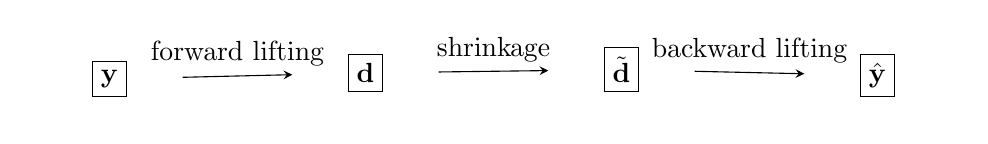
\begin{tikzpicture}
\matrix (m) [matrix of math nodes,row sep=3em,column sep=4em,minimum width=5.25em]
{
	%F_t(x) & F(x) \\
	%A_t & A 
	\framebox[2\width]{$\mathbf{y}$} & \framebox[2\width]{$\mathbf{d}$} & \framebox[2\width]{$\tilde{\mathbf{d}}$} & \framebox[2\width]{$\hat{\mathbf{y}}$}\\};
\path[-stealth]
(m-1-1) edge node [above] {forward lifting} (m-1-2)
(m-1-2) edge node [above] {shrinkage} (m-1-3)
%(m-1-2) edge node [below] {(ex. EbayesThresh)} (m-1-3)
(m-1-3) edge node [above] {backward lifting} (m-1-4);
%(m-2-1.east|-m-2-2) edge node [below] {$\mathcal{B}_T$}
%node [above] {$\exists$} (m-2-2)
%(m-1-2) edge node [right] {$\mathcal{B}_T$} (m-2-2);
%edge [dashed,-] (m-2-1);
\end{tikzpicture}
\caption{Illustration of lifting scheme with shrinkage.} \label{fig:tikzpicture01}
\end{figure}

In the proposed streamflow lifting scheme, we use the same shrinkage strategies used in \cite{Nunes2006} and \cite{Knight2009}. There are several types of shrinkage approaches. In this paper, we focus on median thresholding and hard thresholding. They are implemented as \texttt{median} and \texttt{hard} in \texttt{adlift} and \texttt{nlt} package in R.
To use the lifting scheme one must decide the number of scaling coefficients to be kept in the final representation of the initial signal. In addition, the user specifies \texttt{nkeep} in \texttt{adlift} and \texttt{nlt} package in R. In this paper, we always use the fully decomposed result (\texttt{nkeep=2}) in \cite{Knight2009}, which produces $(n-2)$ detail coefficients from length-$n$ dataset. %It can be realized using \texttt{nkeep=2}, which is default number in both R packages. 

\subsection{Smoothing method on the river network}

In this subsection, we briefly summarize the work of \cite{ODonnell2014}. One of the main ideas of \cite{ODonnell2014} is to simplify the information of the given network by using the concept of streamflow segments. They also suggest a penalize spline-based method with spatial, seasonal, temporal, and interaction basis. In this paper, we focus on the analysis of the spatial behavior of pollutants, considering the structure of river networks like (\ref{eq:scattered}). Therefore, we can consider a straightforward spatial additive model like

\begin{equation}\label{eqn:spatialsimpleadditive}
%y_{i} = \mu + m_{s}(s_i) + \varepsilon_{i},
y_{i} = \mu + m_{x}(x_i) + \varepsilon_{i} = g(x_i) + \varepsilon_{i},
\end{equation}
%(그런데 그냥 (1)번 식 그대로 사용해도 될 듯
where the function $m_x$ describes spatial trends.
The main idea of the spline method is to use a set of basis functions to estimate $g$ in Equation (\ref{eq:scattered}). Suppose that we use $p$ basis functions, then the estimator is $\hat{g}(x) = \sum_{j=1}^{p}\beta_{j} \phi_{j}(x)$.
In \cite{ODonnell2014}, they use B-spline basis, which uses polynomial pieces. Under the above setting, a B-spline model can be formulated as $\mathbf{y}=B\boldsymbol{\beta} +\boldsymbol{\varepsilon}$,  where

$$
B
= 
\begin{pmatrix}
\mathbf{1} & B_{s}
\end{pmatrix},
$$
where $B_{s}$ is a design matrix of spatial components, and $n\times p$ vector $\boldsymbol{\beta}$ is a response vector. 
In this paper, we set $p=1+\text{ the number of streamflow units}$. 
The P-spline model in \cite{ODonnell2014} used a penalized version of B-spline model. It minimizes the following penalized sum of squares

\begin{equation}\label{eqn:ODonnellsmoothing}
(\mathbf{y}-B\boldsymbol{\beta})^{T}(\mathbf{y}-B\boldsymbol{\beta}) + \lambda\boldsymbol{\beta}^{T}D^{T}D\boldsymbol{\beta},
\end{equation}
with respect to $\beta$. In short, (\ref{eqn:ODonnellsmoothing}) becomes
\[
\|\mathbf{y} - B\boldsymbol{\beta}\|^{2} +\boldsymbol{\beta}^{T}P\boldsymbol{\beta}.
\]
In Equation (\ref{eqn:ODonnellsmoothing}), $D$ means the penalty matrix makes the differences of $\beta$ values within nearby stream units. According to \cite{ODonnell2014}, the solution of Equation (\ref{eqn:ODonnellsmoothing}) is $\hat{\boldsymbol{\beta}} = (B^{T}B+ \lambda D^{T} D)^{-1}B^{T}\mathbf{y}$, where $\lambda$ is a smoothing parameter. To select the optimal value of $\lambda$, \cite{ODonnell2014} considers $\lambda$ minimizing $\log(\hat{\sigma}^{2}) + 1 + \frac{2+2\text{dof}}{n-\text{dof}-2}$, where $\text{dof}$ is degree of freedom..
For more information, \cite{ODonnell2014} gives a detail of smoothing methods in the stream network. %To find an optimal $\lambda$, we 
%p의 갯수 아마 맞는 듯

\begin{figure}
	%\centering\includegraphics[height=5.5cm]{Node(small).pdf}\caption{A simple flow-stream data.}
	\centering\includegraphics[width=0.35\textwidth]{Stream_result/Node-flow-complexed2-3.pdf}
	\vspace{-6mm}
	\caption{A simple streamflow data. Five solid black lines represent streme segments,  indexed by $A,B,C,D,$ and $E$. Each line segment has its flow volume, called $f_{A}, f_{B}, \ldots, f_E$. We denote $y_{A}, \ldots y_{E}$ to represent water quality values. }%There are five observation points from $A$ to $E$, located in different segments.}
	\label{fig:nodedescription}
\end{figure}

%For comparison, we consider the flexible approach of \cite{ODonnell2014}. The main idea of \cite{ODonnell2014} is to represent signal part $m$ of (\ref{eqn:simplemodel}) with an additive model based on penalized splines, minimizing
%\[
%\|\mathbf{y} - B\boldsymbol{\beta}\|^{2} +\boldsymbol{\beta}^{T}P\boldsymbol{\beta},
%\label{eqn:Odonnell}
%\]
%where $\mathbf{y}$ is a data vector, $B$ is a basis matrix that is constructed by an additive combination of spatial, temporal, and seasonal basis functions, $P$ is a penalty matrix, and $\boldsymbol{\beta}$ is a set of coefficients. They employ B-splines and estimate $m$ as a linear combination of spatial, temporal, and seasonal B-spline basis functions $\phi_{j}$, i.e., $\hat{m}(x)=\sum_{j}\beta_{j}\phi_{j}(x)$. 

\section{Geum-River TOC data}\label{sec:data}

%NIER address: (http://water.nier.go.kr/),
The data used in this paper are observed in the Geum-River basin, which is located in the central part of South Korea. See Figure \ref{fig:studyarea} (a). According to the Water Environment Information System, operated by the Ministry of Environment in Korea, the Geum-River basin is divided by 14 sub-regions called catchments. All 14 catchments are also divided into several sub-catchments, which are plotted as dotted lines in Figure \ref{fig:studyarea} (a) and (b). %They are used in Section \ref{sec:streamflowrealdata} to construct network clusters for the proposed nondecimated lifting scheme.
Among them, Miho-Cheon catchment marked by orange in Figure \ref{fig:studyarea} (b) is one of the sub-regions. It contains many observational stations compared to other catchments, and there are several cities and factories around it. We believe that taking a closer look at this area is meaningful. We also applied this river network to construct the network model of the simulation study in Section \ref{sec:streamflowsimulationdata}.

The orange lines in the Miho-Cheon catchment of Figure \ref{fig:studyarea} (b) denote streamflow segments which are defined as lines between junctions in a stream network \citep{VerHoef(2006), VerHoef(2010)}. We note that the Miho-Cheon catchment has 113 streamflow segments and 28 observation stations. %total 갯
In total, the Geum-River network has 942 streamflow segments and 127 observation points.

Figure \ref{fig:studyarea} (c) shows populations of cities, counties, and districts located in the Geum-River basin. Note that these administrative area does not fully match to the streamflow segments. From Figure \ref{fig:studyarea} (c), we can check that most of the populations are concentrated on the Northern and Central parts of the Geum-River basin. Figure \ref{fig:studyarea} (d) shows the locations of industrial areas in Geum-River basins. Note that general, national, and urban industrial sites are gathered in Miho-Cheon and its nearby area. Therefore, we can conjecture that many water pollutants will be produced in Miho-Cheon and its nearby river basin.
%(출처 작성 필)

\begin{figure}
	\centering\includegraphics[width=\textwidth]{Stream_result/Studyarea_small.pdf}\\
	\includegraphics[width=\textwidth]{Stream_result/Studyarea_additional.pdf}\caption{(a) Map of Geum-River basin in South Korea. Geum-River catchments are represented in red lines. (b) Enlarged figure of (a). Colored lines denote Geum-River stream networks and black dots are 127 observation points. (c) Populations (2017/12/31, thousands) in Geum-River basin. Gray lines mean cities. (d) Four types  of industrial areas in Geum-river basins in 2018.}
	\label{fig:studyarea}
	%code00_readshp.R (800*400)
	%NIER address: (http://water.nier.go.kr/),
	%code00_readshp.R이 현재 실행 오류가 나고 있기 때문에 다시 한 번 체크해야 -> googlemap 계정 갱신하였
\end{figure}


%(여기서는 spatial data analysis를 하고 있기 때문에 중요치 않다고 생각하면 생략해도 된다)
%\begin{figure}
%	\centering\includegraphics[width=0.8\textwidth]{Miho25A.pdf}
%	\vspace{-4mm}
%	\caption{Total oxidized nitrogen (TN) time series observed at two different observation stations, (a) Miho-Cheon 2  and (b) Miho-Cheon 5A.}
%	\label{fig:TONseries}
%\end{figure}
%
%Figure \ref{fig:TONseries} shows two time series of total oxidized nitrogen (TN) observed at two different stations, Miho-Cheon 2 and Miho-Cheon 5A. Among 28 stations, TN is monthly observed at 15 stations (including Miho-Cheon 2 station) and is weekly observed in 23 stations (including Miho-Cheon 5A station).



\section{Streamflow lifting scheme}\label{sec:streamflowliftingscheme}

In this section, we present our procedure to construct a new lifting scheme for streamflow data by modification of LOCAAT algorithm of  \citet{Jansen2009} that reflects some features of streamflow data. 
Our main idea is to develop a multiscale concept in the streamflow data by incorporating the idea of \cite{Nunes2006} into \cite{ODonnell2014}.
The idea of the streamflow lifting scheme are (i) performing a network-adaptive neighborhood selection, (ii) constructing a prediction filter with flow-adaptive weighted averages, and (iii) determining a removal order by defining a proper contribution measure of each observation point for the stream network.

For a better presentation, we consider a toy example network plotted in Figure \ref{fig:nodedescription}. Suppose that there are five observation points ($A$, $B$, $C$, $D$, $E$) located at different stream segments of a river network. Assume that each segment has a flow volume of $f$. Let $f_A, f_B, \ldots, f_E$ denote flow volume of station $A, B,\ldots, E$. We further denote $y_A, \ldots, y_E$ as water quality observation values at station $A,\ldots, E$.


\subsection{Neighborhood selection}\label{subsec:nbd}

%이것의 복잡한 network 성질 때문에 기존 방법대로 removal order를 정하는 것이 쉽지 않다.

%In this subsection, the concept of Shreve stream order and flow-connected are provided.


%Stream distance of segment $i$ can be measured as the shortest distance between the segment $i$ and the mouth of the river.
%
%(upstream, downstream)

The concept of ``flow-connected" introduced in \cite{VerHoef(2006)} is useful to construct a neighborhood set of a point in stream network. %Although there are some variations to decide the flow-connected, we follow the ``tail-up" approach, according to  \cite{VerHoef(2006)}. 
\cite{VerHoef(2006)} defined that two locations are connected when the intersection of upstreams of two stations is a non-empty set. In our example, segments $A, C$ and $B, C$ are ``flow-connected'' because the water in $A$ and $B$ can go to location $C$. On the other hand, $C$ and $D$ are not flow-connected since the water in $C$ cannot go to station $D$, or vice versa. 

We now use this concept of ``flow-connected'' to decide whether two segments are neighbors or not. In this study, when two points are flow-connected, we consider that they are neighbors of each other.  In Figure \ref{fig:nodedescription}, suppose that we are interested in removing point $C$ at a specific resolution level. By following the concept of flow-connected, we define $A, B$, and $E$ (blue circles) as  its neighborhood, while $D$ (green triangle) is excluded from the neighborhood of $C$.
% For example, in Figure \ref{fig:nodedescription}, neighbors of point $C$ are $A, B,$ and $E$.

One of the distinct characteristics of the proposed neighborhood selection is that it considers both upstream and downstream neighborhoods. By doing so, it can reduce the number of boundary points. At first glance, including downstream points into neighborhood seems awkward. However, by combining an appropriate prediction filter construction explained in Section \ref{subsec:pf}, it is able to generate reasonable prediction filters.

\subsection{Construction of prediction filter }\label{subsec:pf}

In this subsection, we consider a problem of prediction filter construction. The simplest prediction filter is constructed using an equally weighted valued vectors. However, every stream network has its mainstream and substreams. It is plausible that observation values on the mainstream usually has more powerful effect to the nearby observation values. Therefore, the impact of each stream onto the given segment should be different. To consider the influence, it is reasonable to consider the flow volumes.
The main idea of the proposed prediction filter construction is to consider the amount of flow volumes compared to others, where \cite{ODonnell2014} called it as ``relative flow volumes".

Suppose that we have neighbors of a specific point in the stream network. The simplest way to assign weights is to give an equal weight for all neighbors, which may not be desirable. For example, in the case that $f_A$ is much bigger than $f_B$,  $y_A$ has a more massive impact on $y_C$, compared to $y_B$. Also, if $f_D$ is bigger than $f_C$, then $y_E$ is much more different from $y_C$. Thus, we would like to construct flow-adaptive weights that reflect the above consideration. 
%To decide the neighborhood of a specific spatial network point, we should consider a concept of moving average.

%(Shreve stream order)

%We can categorize the stream according to their position. Stream order is used to describe a stream and it make us to divide the stream into several components.

%Although we define neighbors in Section \ref{subsec:nbd}, it is not desirable to give an equal weight for all neighbors. For example, if $f_A$ is much bigger than $f_B$, then $y_A$ has a larger impact on $y_C$, compared to $y_B$. Also, if $f_D$ is bigger than $f_C$, then $y_E$ is much more different from $y_C$. Besides, we need to fix the sum of all weights are equal to one for the stability problem. In this subsection, we adopt flow-adaptive weights construction to solve these problems.




%\subsection{Neighborhood selection}
In the previous toy example of Figure \ref{fig:nodedescription}, suppose that we predict the response value of point $C$ with its neighbors. Since $f_{C}= f_{A}+ f_{B}$, flow-adaptive weights for point $C$ can be defined as ratios of flows, 
\begin{equation}
w_{A} = \frac{f_{A}}{f_{C}},~~w_{B}=\frac{f_{B}}{f_{C}}, ~\text{ and }~ w_{E}=\frac{f_{C}}{f_{E}}.
\label{eqn:flowadaptiveweight}
\end{equation}
Then we obtain a predicted value of $y_{C}$ as $\hat{y}_{C} = \tilde{w}_{A}y_{A} + \tilde{w}_{B}y_{B} + \tilde{w}_{E}y_{E},$  where
\begin{align}
\tilde{w}_{A} &= \frac{f_{A}/f_{C}}{f_{A}/f_{C} + f_{B}/f_{C} + f_{C}/f_{E}},\nonumber\\
\tilde{w}_{B} &= \frac{f_{B}/f_{C}}{f_{A}/f_{C} + f_{B}/f_{C} + f_{C}/f_{E}}, \text{ and } \label{eqn:streamliftingweight}\\
\tilde{w}_{E} &= \frac{f_{C}/f_{E}}{f_{A}/f_{C} + f_{B}/f_{C} + f_{C}/f_{E}}.\nonumber
\end{align}
Therefore, the predicted value of the segment $C$, $\hat{y}_{C}$ is
\begin{equation}
\hat{y}_{C}  = \tilde{w}_{A}y_{A} + \tilde{w}_{B}y_{B} + \tilde{w}_{E}y_{E}.
\label{eqn:sliftingprediction}
\end{equation}

Note that $\tilde{w}_A, \tilde{w}_B,$ and $\tilde{w}_E$ denote normalized flow-adaptive weights to make the sum of weights to be 1, i.e., $\tilde{w}_A + \tilde{w}_B + \tilde{w}_E = 1$. Hence, it is able to construct a lifting scheme for streamflow data by combining flow-adaptive weights of (\ref{eqn:flowadaptiveweight}) and (\ref{eqn:streamliftingweight}) into the conventional lifting scheme. %To decide the densest sampled regions, %consider weighted average of the flow volume, i.e., region of the segment $A$ is $I_{A}=\text{length}_A \times f_A$.
%set the region is proportional to $f$.

In practice, it is uncommon that one knows all $f$ values throughout the entire streamlines. Hence, it is necessary to estimate flow values. For example, in \cite{VerHoef(2006)}, they used an simple equal weight for each split.% by $\sqrt{1/2}$. 
In this study, we assume that flow volume $f$ of the most upstream segments is proportional to their Shreve stream order and segment length. Stream order is a positive whole number frequently used in hydrology to define stream-based distance in a stream network system. There are various kinds of stream order. Among them, the Shreve stream order is one of the most straightforward stream orders \citep{Cressie2006, VerHoef(2010)}. \cite{Cressie2006} defined the stream order as merely a count of the number of sources in the upstream portion of a stream network. Shreve stream order starts from setting all upper segments to 1. Magnitudes increase at all junctions in the stream network system. For example, if a stream has magnitude 1 and it combines with a new stream having magnitude 2, that has magnitude 3. By doing so, it is able to construct all magnitudes of the given network.

%In this chapter, If we let the stream order of the upper-most segments (describe in Figure \ref{fig:clusterconstruction}) is 1, 
In this paper, we approximate $f$ values by following the definition of Shreve stream order above and additionally letting the flow of the upper-most segments be proportional to their lengths to prevent multiple tie values in flow volumes.
%By following the definition of Shreve stream order above and letting the flow of the upper-most segments be proportional to their lengths, 
After defining flow volumes of upper-most segments, one can define a flow volume of the next upstream segments as a sum of their upstream segments. %The construction is exactly the same as in Shreve order construction.
By repeating this approach, we obtain all $f$ values in the stream network. In this paper, we assume that we know flow volume related weights, which generates by $\log(\sqrt{f})$ values. By following the \cite{ODonnell2014}, we normalize all $\log(\sqrt{f})$ values are lying between $0.2$ to $1.5$.
	
%Furthermore, by following the \cite{ODonnell2014}, we use $\log(\sqrt{f})$ values, after normalizing all $\log(\sqrt{f})$ values are lying between $0.2$ to $1.5$.}

%(consider only the final point)., described in Figure \ref{fig:clusterconstruction}, 

%\subsection{Removal orders}

\subsection{Removal point selection}

For the streamflow lifting scheme, it is necessary to decide the removal order. In the case that the data lie in the real line such as Figure \ref{fig:removeI}, it is easy to adapt a conventional approach such as \cite{Nunes2006}. They used the length of a point in real line for the computation of an integral. It can be extended in the two-dimensional data, suggested by \cite{Jansen2009}. The basic idea of \cite{Jansen2009} to decide the removal point is setting an appropriate integral of a scaling function to find the densest observation in the Euclidean domain. \cite{Jansen2009} suggested Voronoi-polygon based area measurement as a candidate of a proper integral and selected a point that has the smallest integral as a removal point in LOCAAT algorithm.

However, these methods cannot be directly applicable to the streamflow data since the network is not easily projected onto one or two-dimensional data. Here, we suggest a simple approach to distinguish which points are located in the densest region of the river network by using the measure of the contribution of each segment in data. We define an integral as a contribution of each observation point to the network.
To define a contribution of each point in streamflow data, we use flow-adaptive weights defined in (\ref{eqn:streamliftingweight}). Consider the simple example described in Figure \ref{fig:nodedescription}. Suppose that at the $j$th level, we want to remove point $C$ with neighborhood points $A, B$, and $E$. Let $I_A^{j}$ denote an integral of point $A$ at the $j$th level, which is defined by the volume of the segment where $A$ is located, say $V_A$. We define the volume $V$ as a product of flow $f$ and length of the segment $\ell$,
%\begin{equation}
%I_A^{j} = V_A = f_A\times l_A.
%\end{equation}
\begin{align}
I_A^{j} &= V_A = f_A\times \ell_A,\nonumber\\
I_B^{j} &= V_B = f_B\times \ell_B, \text{ and }\\
I_E^{j} &= V_E = f_E\times \ell_E.\nonumber
\end{align}
%In the same way, we can define $I_{B}^{j}$ and $I_{E}^{j}$.

At the next level, $j-1$ after point $C$ is removed, we need to update the integral of neighborhood points. For this purpose, we use a weighted volume of the point $C$ according to the weights of neighbors in (\ref{eqn:streamliftingweight}). Thus, $I_A^{j}, I_{B}^{j},$ and $I_E^{j}$ are updated to
\begin{align}
I_A^{j-1}&=I_A^{j} + \tilde{w}_A\times V_C,\nonumber\\
I_B^{j-1}&= I_B^{j} + \tilde{w}_B \times V_C, \text{ and }\\
I_E^{j-1} &= I_E^{j} + \tilde{w}_E \times V_C.\nonumber
\end{align}
%$I_A^{j-1}=I_A^{j} + \tilde{w}_A\times V_C, I_B^{j-1}= I_B^{j} + \tilde{w}_B \times V_C$ and $I_E^{j-1} = I_E^{j} + \tilde{w}_E \times V_C$. 
Note that since $\tilde{w}_A\times V_C +\tilde{w}_B \times V_C+ \tilde{w}_E \times V_C=I_C^{j}$, the sum of integrals is not changed. For the point to be removed at the $j-1$th level, we select a point that has the minimum value of $I^{j-1}$. For the update filter, we use the minimum norm solution based filter in (\ref{eqn:updatefilter}).

\subsection{Nondecimated lifting scheme for streamflow data}

As mentioned in Section \ref{subsec:otherlifting}, sometimes we can reduce the mean squared error of the lifting scheme in a nonparametric regression setting by considering a nondecimated version of the lifting scheme. In this paper, we applied a similar approach to the streamflow data. In this paper, we assume that the current stream distance-based removal is one of the well-behaved trajectories from minimizing the root mean squared error perspective. Then we generate multiple trajectories produced from permutations. Permutations are only performed within the same sub-catchment regions, which are dotted lines in Figure \ref{fig:studyarea}. In this paper, we fixed the number of permutations \texttt{Q=10}. To generate such well-behaved trajectories, we define clusters first and do permutation to observations located in the same cluster.

In this paper, we consider two kinds of tuning parameters: (i) the number of trajectories (\texttt{Q=10}) and (ii) the number of permutation within single trajectory (\texttt{v=5}) Note that we can have the same denoising results when we use \texttt{Q=10} and \texttt{v=0}.

%\textcolor{red}{Note that in nondecimated version of lifting scheme, it is not easy to construct multiresolution representation.}
%nondecimated version에 대한 추가 설명 필요. ``well-behaved''에 대한 설명 추가 필요

\section{Simulation study}\label{sec:streamflowsimulationdata}

%Suppose that the data are observed from the following regression model,
%\begin{equation}
%y_{i} = g_{i}+\varepsilon_{i},
%\label{eqn:simplemodel}
%\end{equation}
%%where $c=5$ is a constant, 
%where $g_i=g(x_i)$ is the true signal at the $i$th stream segment and $\varepsilon_{i}$ denote error terms. %\cite{ODonnell2014} used the same model for the analysis of their Tweed data. 

\begin{figure}
	%\centering\includegraphics[width=0.8\textwidth]{Stream_cluster_maps_new.pdf}
	\centering\includegraphics[width=1\textwidth]{Stream_result/Stream_cluster_maps_new(4).pdf}
	\centering\includegraphics[width=1\textwidth]{Stream_result/Stream_cluster_maps_STPCA.pdf}
	\vspace{-10mm}\caption{(a) Cluster construction (red circles) on the Miho-Cheon stream network. We classify streamflow segments into two, upper-most segments (purple squares) and non-upper-most segments (orange circles). (b) Colors represent substreams for the sampling procedure. The sampling probability is proportional to the number of streams of each substream.} %(When \texttt{nkeep=2})}
	\label{fig:clusterconstruction}
\end{figure}

In this section, we conduct numerical experiments for the evaluation of our approach for spatial streamflow data analysis. Suppose that the data are observed from the regression model in Equation \ref{eq:scattered}. We mainly focus on the situation that the underlying mean-field of the data is piecewise constant. Therefore, there are several discontinuous function values in a stream network, which sometimes fails to have an appropriate estimation using conventional smoothing-based methods. For comparison, we consider the flexible smoothing approach of \cite{ODonnell2014}. For the proposed approach, we consider three kinds of different methods: ordinary streamflow lifting scheme with median thresholding (\texttt{S-Lifting (M)}), ordinary streamflow lifting scheme with hard thresholding (\texttt{S-Lifting (H)}), and nondecimated streamflow lifting scheme with median thresholding (\texttt{S-Lifting (N)}).

For simulation setup, we consider two types of stream networks: one is the Miho-Cheon streamflow segments (Figure \ref{fig:clusterconstruction} (a) and (b)), and the other is a simulated river network used in \cite{Gallacher2017} (Figure \ref{fig:clusterconstruction} (c) and (d)). Each network consists of 113 and 80 stream segments.  For each river network, we classify whole stream segments into two groups, upper-most segments and non-upper most segments, shown in Figure \ref{fig:clusterconstruction} (a). %Note that there are 55 upper-most segments in the streamflow network. 
We assume that there are no intrinsic sources to change the simulated signal values. Then the signal values of non-upper-most segments are generated from a weighted average of nearby upstream signal values of upper-most segments. It implies that it is enough for the simulation only to generate signal values of upper-most segments. 

Moreover, we divide upper-most segments into a few clusters, shown in Figure \ref{fig:clusterconstruction}, to generate inhomogeneous stream network data. We assume that within a cluster, all segments have the same signal value. For each simulated data set, $g(x_i)$ values of upper-most segments are  generated as follows: (i) all $g(x_i)$ values of upper-most segments are set to be 9, (ii) a cluster is randomly selected from the clusters in Figure  \ref{fig:clusterconstruction}, and (iii) $g(x_i)$ values in the selected cluster are replaced with a values that is randomly chosen from 12, 15, 18. This procedure is repeated until at least 30 upper-most segments have a value bigger than 9. An example of the simulated data generation is plotted in Figure \ref{fig:streamsimresult} (a).
%\begin{enumerate}
%	\item We set all $g(x_i)$ value of upper-most segments 4.
%	\item We randomly select a cluster, which is described in Figure  \ref{fig:clusterconstruction}, and assign a value which is one of three: 7, 10, 13. This procedure is repeated until at least 30 upper-most segments have a value bigger than 4.
%\end{enumerate}

%\begin{enumerate}
%	\item 
%\end{enumerate}

%\begin{algorithm}[H]
%	\caption{Generate $m_{j}(x_{i})$ values for upper-most segments}\label{alg:IT-VMD2}
%	\begin{algorithmic}[1]
%		\State Set a vector of signal values to make differences, $\mathbf{m}$. Let $\mathcal{J}$ is the collection of predetermined clusters shown in Figure \ref{fig:clusterconstruction} (a). Let $n$ is the number of segments samples to use the data analysis. Let $I$ is the set of segments which are selected. Initially, $I=\emptyset$.
%		\State (Initial attempt) Randomly select $|\mathbf{m}|$ clusters from $\mathcal{J}$ and assign signal values. Let $J_{1},\ldots, J_{|\mathbf{m}|}$ are selected clusters. we update the set $\mathcal{J}=\mathcal{J}\backslash (J_{1}\cup\ldots \cup J_{|\mathbf{m}|})$ and $I=I\cup \{i, i\in J_{1}\cup\ldots \cup J_{|\mathbf{m}|}\}$.
%		\State Repeat followings while $|I|\leq n$. % $\sum_{r=1}^{R}|\mathcal{P}_{r}| \leq |\mathcal{P}_{r_{\text{opt}}}|$. 
%		\begin{itemize} 
%			\item[a] Randomly select a cluster from new $\mathcal{J}$. Assign a signal value which has the least number of observations having that value.
%		\end{itemize}
%		\State Return $m_{i,j}(x_{i})$.
%	\end{algorithmic}
%\end{algorithm}
%\endfoil

% In each simulation, to give more variability for each signal, three groups of upstreams are randomly selected, having values $\mathbf{m}=(7,10,13)$. Other non-selected groups have value $m=4$. For the $i$-th segment in the $j$-th upstreams group, 


We further consider three different spatial designs for the simulated data in the stream network. (i) For a sparse design, 40 observation stations located on 40 different segments among the total 113 Miho-Cheon stream segments. A realization is shown in Figure \ref{fig:clusterconstruction} (b). (ii) Eighty stations, which is almost two-thirds of the number of Miho-Cheon streams.  (iii) As for a dense case, 113 stations are considered. Along the same lines, we analyze the simulated network of \cite{Gallacher2017} in two situations, (i) suppose that we only have observations in 40 stations, and (ii) we have one observation at each segment. 

%(원래 글)
%We further consider three different spatial designs for the simulated data in the river network. (i) For a sparse design, 28 observational stations are located on 26 segments among 113 streamflow segments. This case exactly reflects the real data in Miho-cheon catchment. (ii) 60 stations including 28 stations in (i) are located on 58 segments, which is almost half of the number of Miho-cheon streams. A realization is shown in Figure \ref{fig:clusterconstruction} (b). (iii) As for a dense case, 115 stations including 28 stations in (i) are located on 113 segments. 


%Typically, we have a relatively small number of observations compared to the number of streams in a river network. Note that in Miho-cheon catchment, 28 observational stations are located on 26 segments among 113 streamflow segments. To reflect this reality, we design the simulated data that are observed at 60 stations located on 58 segments, which is almost half of the number of Miho-cheon streams. {\color{red}Furthermore, in the sampling procedure, we consider the predetermined substreams, described in \ref{fig:clusterconstruction} (b), to prevent an awkward sampling result. How ?}



%follows:  (a) the observed values are available in 28 stations, where locations are the same as in the real data of Miho-cheon area. (b) Second, we additionally select 32 segments and assume that we have available 60 data on 58 segments, which is almost half of the number of Miho-cheon streams. Within the sampling procedure, we consider the predetermined substreams, described in \ref{fig:clusterconstruction} (b), to prevent an awkward sampling result.
%proportional to predetermined substreams. 
%One of the realizations is represented in Figure \ref{fig:clusterconstruction} (b). Third, we assume that we have at least one observation for all 113 segments, including 28 observations. In this case, we have 115 observations.


The noise terms are generated from $\varepsilon_{i} \stackrel{\text{i.i.d.}}{\sim} \mathcal{N}(0,\sigma^{2})$ with (i) $\sigma=0.5$, (ii) $\sigma=1$, and (iii) $\sigma=1.5$. As for evaluation measure, we consider the root mean square error (RMSE) as 
\begin{equation}\label{eq:RMSE}
\text{RMSE}=\sqrt{\frac{\sum_{i=1}^{N_{tot}} (g(x_i)-\hat{g}(x_i))^{2}} {N_{tot}}},
\end{equation}
where $\hat{g}(x_i)$ is an estimated smoothed value at segment $i$, and $N_{tot}$ means the total number of stream segments in the river network. For each combination of three spatial designs and two $\sigma$'s, we compute RMSE values according to our method and the approach of \cite{ODonnell2014} over 100 simulated data sets. Table \ref{table:streamsimresult} lists the RMSE values. As listed, the proposed method outperforms the approach of \cite{ODonnell2014} for all the combinations. For visual inspection, we look at fitting results of the spatial design with 60 stations and $\sigma=1$ shown in Figure \ref{fig:streamsimresult}. The proposed method performs well by reflecting the inhomogeneous features of the underlying field.   





%From (c) of \ref{fig:streamsimresult}, we find that \cite{ODonnell2014}'s method cannot make a denoised result when the variability of the data is inhomogeneous in the spatial domain. However, the proposed method produce smoothed output for all streamflow regions because of its local adaptability. Hence, the output of the streamflow lifting scheme is similar to true underlying streamflow signals. We also note that the standard error of the proposed method is always larger than B-spline based method. We conjecture that if the number of observation is larger than that of the simulation setting, it would be reduced.


% Please add the following required packages to your document preamble:
% \usepackage{multirow}
%\begin{table}[]
%	\centering
%	\caption{RMSE of simulation result (and their standard error). In each simulation, the number of iterations is 100.}
%	\label{table:streamsimresult}
%	\resizebox{\textwidth}{!}{\begin{tabular}{|c|c|c|c|c|c|c|c|c|c|}
%		\hline
%		\multirow{2}{*}{\begin{tabular}[c]{@{}c@{}}RMSE\\ (Std. error)\end{tabular}} & \multicolumn{3}{c|}{Obs=40}                                                                                                                                                                                  & \multicolumn{3}{c|}{Obs=80}                                                                                                                                                                                  & \multicolumn{3}{c|}{Obs=113}                                                                                                                                                                                 \\ \cline{2-10} 
%		& $\sigma=1$                                                         & $\sigma=1.5$                                                       & $\sigma=2$                                                         & $\sigma=1$                                                         & $\sigma=1.5$                                                       & $\sigma=2$                                                         & $\sigma=1$                                                         & $\sigma=1.5$                                                       & $\sigma=2$                                                         \\ \hline
%		O'Donnell                                                                    & \begin{tabular}[c]{@{}c@{}}2.0801\\ (0.1968)\end{tabular}          & \begin{tabular}[c]{@{}c@{}}2.1952\\ (0.2377)\end{tabular}          & \textbf{\begin{tabular}[c]{@{}c@{}}2.3415\\ (0.2567)\end{tabular}} & \begin{tabular}[c]{@{}c@{}}1.5355\\ (0.1539)\end{tabular}          & \begin{tabular}[c]{@{}c@{}}1.6757\\ (0.1582)\end{tabular}          & \begin{tabular}[c]{@{}c@{}}1.7808\\ (0.1802)\end{tabular}          & \begin{tabular}[c]{@{}c@{}}1.3159\\ (0.1268)\end{tabular}          & \begin{tabular}[c]{@{}c@{}}1.4579\\ (0.1293)\end{tabular}          & \begin{tabular}[c]{@{}c@{}}1.5927\\ (0.1432)\end{tabular}          \\ \hline
%		\begin{tabular}[c]{@{}c@{}}Proposed\\ (Median)\end{tabular}                  & \begin{tabular}[c]{@{}c@{}}1.7113\\ (0.4140)\end{tabular}          & \begin{tabular}[c]{@{}c@{}}2.0667\\ (0.4824)\end{tabular}          & \begin{tabular}[c]{@{}c@{}}2.4170\\ (0.4734)\end{tabular}          & \begin{tabular}[c]{@{}c@{}}1.0901\\ (0.1828)\end{tabular}          & \textbf{\begin{tabular}[c]{@{}c@{}}1.3969\\ (0.2082)\end{tabular}} & \textbf{\begin{tabular}[c]{@{}c@{}}1.6578\\ (0.3031)\end{tabular}} & \textbf{\begin{tabular}[c]{@{}c@{}}0.8496\\ (0.1335)\end{tabular}} & \textbf{\begin{tabular}[c]{@{}c@{}}1.1780\\ (0.1747)\end{tabular}} & \textbf{\begin{tabular}[c]{@{}c@{}}1.4597\\ (0.2204)\end{tabular}} \\ \hline
%		\begin{tabular}[c]{@{}c@{}}Proposed\\ (Hard)\end{tabular}                    & \textbf{\begin{tabular}[c]{@{}c@{}}1.6134\\ (0.3901)\end{tabular}} & \textbf{\begin{tabular}[c]{@{}c@{}}2.0101\\ (0.4559)\end{tabular}} & \begin{tabular}[c]{@{}c@{}}2.3973\\ (0.4156)\end{tabular}          & \textbf{\begin{tabular}[c]{@{}c@{}}1.0527\\ (0.1725)\end{tabular}} & \begin{tabular}[c]{@{}c@{}}1.3995\\ (0.1939)\end{tabular}          & \begin{tabular}[c]{@{}c@{}}1.6907\\ (0.2939)\end{tabular}          & \begin{tabular}[c]{@{}c@{}}0.8613\\ (0.1066)\end{tabular}          & \begin{tabular}[c]{@{}c@{}}1.2174\\ (0.1522)\end{tabular}          & \begin{tabular}[c]{@{}c@{}}1.5413\\ (0.2021)\end{tabular}          \\ \hline
%	\end{tabular}}
%	\vspace{-1mm}
%	%data
%	%StreamSim40(sd1)new.RDS, StreamSim40(sd15)new.RDS, , StreamSim40(sd2)new.RDS, StreamSim80(sd1)new.RDS, StreamSim80(sd15)new.RDS, StreamSim80(sd2)new.RDS, StreamSim113(sd1)new.RDS, StreamSim113(sd15)new.RDS, StreamSim113(sd2)new.RDS
%\end{table}

% Please add the following required packages to your document preamble:
% \usepackage{multirow}
\begin{table}[]
	\centering
	\resizebox{\textwidth}{!}{\begin{tabular}{|c|c|c|c|c|c|c|c|c|c|}
			\hline
			\multirow{2}{*}{\begin{tabular}[c]{@{}c@{}}RMSE\\ (Std. error)\end{tabular}} & \multicolumn{3}{c|}{Obs=40}                                                                                                                                                                                  & \multicolumn{3}{c|}{Obs=80}                                                                                                                                                                                  & \multicolumn{3}{c|}{Obs=113}                                                                                                                                                                                 \\ \cline{2-10} 
			& $\sigma=1$                                                         & $\sigma=1.5$                                                       & $\sigma=2$                                                         & $\sigma=1$                                                         & $\sigma=1.5$                                                       & $\sigma=2$                                                         & $\sigma=1$                                                         & $\sigma=1.5$                                                       & $\sigma=2$                                                         \\ \hline
			O'Donnell                                                                    & \begin{tabular}[c]{@{}c@{}}2.0988\\ (0.1957)\end{tabular}          & \begin{tabular}[c]{@{}c@{}}2.2101\\ (0.2052)\end{tabular}          & \textbf{\begin{tabular}[c]{@{}c@{}}2.2882\\ (0.2317)\end{tabular}} & \begin{tabular}[c]{@{}c@{}}1.5270\\ (0.1561)\end{tabular}          & \begin{tabular}[c]{@{}c@{}}1.6336\\ (0.1513)\end{tabular}          & \begin{tabular}[c]{@{}c@{}}1.7542\\ (0.1654)\end{tabular}          & \begin{tabular}[c]{@{}c@{}}1.3252\\ (0.1364)\end{tabular}          & \begin{tabular}[c]{@{}c@{}}1.4458\\ (0.1320)\end{tabular}          & \begin{tabular}[c]{@{}c@{}}1.5798\\ (0.1609)\end{tabular}          \\ \hline
			\begin{tabular}[c]{@{}c@{}}Proposed\\ (Median)\end{tabular}                  & \begin{tabular}[c]{@{}c@{}}1.7089\\ (0.4181)\end{tabular}          & \begin{tabular}[c]{@{}c@{}}2.1410\\ (0.5202)\end{tabular}          & \begin{tabular}[c]{@{}c@{}}2.3588\\ (0.5134)\end{tabular}          & \begin{tabular}[c]{@{}c@{}}1.0662\\ (0.1877)\end{tabular}          & \begin{tabular}[c]{@{}c@{}}1.3488\\ (0.2343)\end{tabular} & \begin{tabular}[c]{@{}c@{}}1.6377\\ (0.2686)\end{tabular} & \begin{tabular}[c]{@{}c@{}}0.8362\\ (0.1187)\end{tabular} & \begin{tabular}[c]{@{}c@{}}1.1656\\ (0.1929)\end{tabular} & \begin{tabular}[c]{@{}c@{}}1.4141\\ (0.2119)\end{tabular} \\ \hline
			\begin{tabular}[c]{@{}c@{}}Proposed\\ (Hard)\end{tabular}                    & \textbf{\begin{tabular}[c]{@{}c@{}}1.6287\\ (0.3882)\end{tabular}} &
			\begin{tabular}[c]{@{}c@{}}2.1281\\ (0.4913)\end{tabular} & \begin{tabular}[c]{@{}c@{}}2.3647\\ (0.4704)\end{tabular}          & \textbf{\begin{tabular}[c]{@{}c@{}}1.0382\\ (0.1528)\end{tabular}} & \begin{tabular}[c]{@{}c@{}}1.3440\\ (0.1903)\end{tabular}          & \begin{tabular}[c]{@{}c@{}}1.6400\\ (0.2524)\end{tabular}          & \begin{tabular}[c]{@{}c@{}}0.8386\\ (0.1074)\end{tabular}          & \begin{tabular}[c]{@{}c@{}}1.2142\\ (0.1569)\end{tabular}          & \begin{tabular}[c]{@{}c@{}}1.5172\\ (0.1985)\end{tabular}          \\ \hline
			\begin{tabular}[c]{@{}c@{}}Proposed\\ (Median, nlt)\end{tabular}                    & \begin{tabular}[c]{@{}c@{}}1.7210\\ (0.3907)\end{tabular} & \textbf{\begin{tabular}[c]{@{}c@{}}2.1143\\ (0.4517)\end{tabular}} & \begin{tabular}[c]{@{}c@{}}2.3292\\ (0.4460)\end{tabular}          & \begin{tabular}[c]{@{}c@{}}1.0428\\ (0.1849)\end{tabular}  & \textbf{\begin{tabular}[c]{@{}c@{}}1.3212\\ (0.2241)\end{tabular}}          & \textbf{\begin{tabular}[c]{@{}c@{}}1.6076\\ (0.2588)\end{tabular}}          & \textbf{\begin{tabular}[c]{@{}c@{}}0.8000\\ (0.1158)\end{tabular}}          & \textbf{\begin{tabular}[c]{@{}c@{}}1.1225\\ (0.1760)\end{tabular}}          & \textbf{\begin{tabular}[c]{@{}c@{}}1.3705\\ (0.2081)\end{tabular}}          \\ \hline
	\end{tabular}}
	\caption{RMSE of simulation result (and their standard error). In each simulation, the number of iterations is 100.}
	\label{table:streamsimresult}
	\vspace{-1mm}
	%data
	%StreamSim40(sd1)nlt.RDS, StreamSim40(sd15)nlt.RDS, , StreamSim40(sd2)nlt.RDS, StreamSim80(sd1)nlt.RDS, StreamSim80(sd15)nlt.RDS, StreamSim80(sd2)nlt.RDS, StreamSim113(sd1)nlt.RDS, StreamSim113(sd15)nlt.RDS, StreamSim113(sd2)nlt.RDS
\end{table}





%\begin{figure}
%	%\centering\includegraphics[width=0.8\textwidth]{Stream_Sim_Result_New3.png}
%	\centering\includegraphics[width=0.95\textwidth]{SLifting_Comp_01.png}
%	\vspace{-4mm}\caption{(a) True signals, (b) noisy observed values when $\text{Obs=60}$, (c) estimation results of \cite{ODonnell2014} and (d) the proposed method with median thresholding, (e) hard thresholding and (f) median with nondecimated methods.} %(When \texttt{nkeep=2})}
%	\label{fig:streamsimresult}
%\end{figure}


\begin{figure}
	%\centering\includegraphics[width=0.8\textwidth]{Stream_Sim_Result_New3.png}
	\centering\includegraphics[width=0.95\textwidth]{Stream_Result/SLifting_Comp_02.png}
	\vspace{-4mm}\caption{(a) True signals, (b) noisy observed values when $\text{Obs=40}$, (c) estimation results of \cite{ODonnell2014}, (d) the proposed method with median thresholding, (e) with hard thresholding and (f) the proposed nondecimated method with median thresholding.} %(When \texttt{nkeep=2})}
	\label{fig:streamsimresult}
	%penalty term estimation result:
	%[1] 22.44695 50.00000 25.00000  5.00000 50.00000 25.00000  5.00000 25.00000
	%[9] 25.00000
\end{figure}


\begin{figure}
	%\centering\includegraphics[width=0.8\textwidth]{Stream_Sim_Result_New3.png}
	\centering\includegraphics[width=0.95\textwidth]{Stream_Result/SLifting_Comp_03.png}
	\vspace{-4mm}\caption{(a) True signals, (b) noisy observed values when $\text{Obs=60}$, (c) estimation results of \cite{ODonnell2014}, (d) the proposed method with median thresholding, (e) with hard thresholding and (f) the proposed nondecimated method with median thresholding.} %(When \texttt{nkeep=2})}
	\label{fig:streamsimresult2}
\end{figure}




%(alternative)


% Please add the following required packages to your document preamble:
% \usepackage{multirow}
%\begin{table}[]
%	\centering
%	\caption{RMSE of simulation result of riverflow network data used in \cite{Gallacher2017} (and their standard error). In each simulation, the number of iterations is 100.}
%	\label{table:streamsimresult2}
%	\resizebox{\textwidth}{!}{\begin{tabular}{|c|c|c|c|c|c|c|}
%		\hline
%		\multirow{2}{*}{\begin{tabular}[c]{@{}c@{}}RMSE\\ (Std. error)\end{tabular}} & \multicolumn{3}{c|}{Obs=40}                                                                                                                                                                                  & \multicolumn{3}{c|}{Obs=80}                                                                                                                                                                                  \\ \cline{2-7} 
%		& $\sigma=1$                                                         & $\sigma=1.5$                                                       & $\sigma=2$                                                         & $\sigma=1$                                                         & $\sigma=1.5$                                                       & $\sigma=2$                                                         \\ \hline
%		O'Donnell                                                                    & \begin{tabular}[c]{@{}c@{}}1.8188\\ (0.3014)\end{tabular}          & \begin{tabular}[c]{@{}c@{}}1.8912\\ (0.2971)\end{tabular}          & \begin{tabular}[c]{@{}c@{}}1.9739\\ (0.3138)\end{tabular}          & \begin{tabular}[c]{@{}c@{}}1.2775\\ (0.1439)\end{tabular}          & \begin{tabular}[c]{@{}c@{}}1.4169\\ (0.1600)\end{tabular}          & \begin{tabular}[c]{@{}c@{}}1.5359\\ (0.2269)\end{tabular}          \\ \hline
%		\begin{tabular}[c]{@{}c@{}}Proposed\\ (Median)\end{tabular}                  & \begin{tabular}[c]{@{}c@{}}1.2061\\ (0.3036)\end{tabular}          & \textbf{\begin{tabular}[c]{@{}c@{}}1.5354\\ (0.3417)\end{tabular}} & \textbf{\begin{tabular}[c]{@{}c@{}}1.7913\\ (0.3998)\end{tabular}} & \begin{tabular}[c]{@{}c@{}}0.7460\\ (0.1546)\end{tabular}          & \textbf{\begin{tabular}[c]{@{}c@{}}1.0415\\ (0.2102)\end{tabular}} & \textbf{\begin{tabular}[c]{@{}c@{}}1.2534\\ (0.2484)\end{tabular}} \\ \hline
%		\begin{tabular}[c]{@{}c@{}}Proposed\\ (Hard)\end{tabular}                    & \textbf{\begin{tabular}[c]{@{}c@{}}1.1743\\ (0.2592)\end{tabular}} & \begin{tabular}[c]{@{}c@{}}1.5828\\ (0.3217)\end{tabular}          & \begin{tabular}[c]{@{}c@{}}1.8808\\ (0.3533)\end{tabular}          & \textbf{\begin{tabular}[c]{@{}c@{}}0.7417\\ (0.1558)\end{tabular}} & \begin{tabular}[c]{@{}c@{}}1.0634\\ (0.2065)\end{tabular}          & \begin{tabular}[c]{@{}c@{}}1.3499\\ (0.2709)\end{tabular}          \\ \hline
%	\end{tabular}}
%	\vspace{-1mm}
%\end{table}



% Please add the following required packages to your document preamble:
% \usepackage{multirow}
\begin{table}[]
	\centering
	\resizebox{\textwidth}{!}{\begin{tabular}{|c|c|c|c|c|c|c|}
			\hline
			\multirow{2}{*}{\begin{tabular}[c]{@{}c@{}}RMSE\\ (Std. error)\end{tabular}} & \multicolumn{3}{c|}{Obs=40}                                                                                                                                                                                  & \multicolumn{3}{c|}{Obs=80}                                                                                                                                                                                  \\ \cline{2-7} 
			& $\sigma=1$                                                         & $\sigma=1.5$                                                       & $\sigma=2$                                                         & $\sigma=1$                                                         & $\sigma=1.5$                                                       & $\sigma=2$                                                         \\ \hline
			O'Donnell                                                                    & \begin{tabular}[c]{@{}c@{}}1.7266\\ (0.2638)\end{tabular}          & \begin{tabular}[c]{@{}c@{}}1.8695\\ (0.2835)\end{tabular}          & \begin{tabular}[c]{@{}c@{}}1.9698\\ (0.2839)\end{tabular}          & \begin{tabular}[c]{@{}c@{}}1.2698\\ (0.1251)\end{tabular}          & \begin{tabular}[c]{@{}c@{}}1.3815\\ (0.1727)\end{tabular}          & \begin{tabular}[c]{@{}c@{}}1.5421\\ (0.2017)\end{tabular}          \\ \hline
			\begin{tabular}[c]{@{}c@{}}Proposed\\ (Median)\end{tabular}                  & \begin{tabular}[c]{@{}c@{}}1.1716\\ (0.2530)\end{tabular}          & \begin{tabular}[c]{@{}c@{}}1.5464\\ (0.3611)\end{tabular} & \begin{tabular}[c]{@{}c@{}}1.8121\\ (0.3539)\end{tabular} & \begin{tabular}[c]{@{}c@{}}0.7265\\ (0.1212)\end{tabular}          & \begin{tabular}[c]{@{}c@{}}1.0249\\ (0.1510)\end{tabular} & \begin{tabular}[c]{@{}c@{}}1.2818\\ (0.2599)\end{tabular} \\ \hline
			\begin{tabular}[c]{@{}c@{}}Proposed\\ (Hard)\end{tabular}                    &\textbf{\begin{tabular}[c]{@{}c@{}}1.1417\\ (0.2244)\end{tabular}} & \begin{tabular}[c]{@{}c@{}}1.5769\\ (0.3050)\end{tabular}          & \begin{tabular}[c]{@{}c@{}}1.9040\\ (0.3286)\end{tabular}          & \begin{tabular}[c]{@{}c@{}}0.7396\\ (0.1317)\end{tabular} & \begin{tabular}[c]{@{}c@{}}1.0666\\ (0.1678)\end{tabular}          & \begin{tabular}[c]{@{}c@{}}1.3705\\ (0.2495)\end{tabular}          \\ \hline
			\begin{tabular}[c]{@{}c@{}}Proposed\\ (Median, nlt)\end{tabular}                    & \begin{tabular}[c]{@{}c@{}}1.1443\\ (0.2494)\end{tabular}          & \textbf{\begin{tabular}[c]{@{}c@{}}1.4988\\ (0.3267)\end{tabular}}          & \textbf{\begin{tabular}[c]{@{}c@{}}1.7329\\ (0.3385)\end{tabular}}          & \textbf{\begin{tabular}[c]{@{}c@{}}0.7162\\ (0.1219)\end{tabular}} & \textbf{\begin{tabular}[c]{@{}c@{}}1.0106\\ (0.1678)\end{tabular}}          & \textbf{\begin{tabular}[c]{@{}c@{}}1.2816\\ (0.2712)\end{tabular}}          \\ \hline
	\end{tabular}}
	\caption{RMSE of simulation result of riverflow network data used in \cite{Gallacher2017} (and their standard error). Note that in each simulation, the number of iterations is 100.}
	\label{table:streamsimresult2}
	\vspace{-1mm}
	%code18_sim_stpca_data_nlt(iter).R
\end{table}

Table \ref{table:streamsimresult} and \ref{table:streamsimresult2} are the RMSE summary of the simulation study. We find that the proposed methods work well under the given simulation settings, especially when $\sigma$ is small. \cite{ODonnell2014}'s method generally gives more robust RMSE compared to proposed methods. When the number of observations is small and the proposed methods usually give a lower RMSE. 
The proposed methods work well under situations that nearby segments have similar values while there are big differences among different streams. On the other hand, the performance of the proposed methods is also dependent on the number of sampling observations. Therefore, when the number of observations is small compared to the number of streamflow segments, it is better to consider both the proposed methods and \cite{ODonnell2014}'s approach.
For the nondecimated version of the proposed lifting scheme, we find that it works well under the simulation setting, which assume that we have knowledge about the behavior of the data. %If we are hard to construct an appropriate set of clusters, it may not work well, as in Section \ref{sec:streamflowrealdata}.


%\section{Real data analysis}\label{sec:streamflowrealdata}
%
%Figure \ref{fig:resultstreamflow} show the result of streamflow lifting scheme applied to Miho-cheon streamflow data residuals. We can find that \cite{ODonnell2014}'s method follows raw residuals, meaning that smoothing is not conducted. In the streamflow lifting scheme, we observe the effect of smoothing with change the estimate of sampling standard deviation of the data, $\hat{\sigma}$. If the value is large, one can get the more smoothed representation of the river network.
%
%For real data analysis, we analyze the data with two-step approach. First, to eliminate temporal variability and seasonality, we fit B-spline smoothing using timewise and seasonal B-spline basis, following work of \citet{ODonnell2014}. After then, we apply the proposed streamflow lifting scheme with residuals of the above step.
%
%The right of Figure \ref{fig:resultstreamflowst} show smoothing results of stream segment 16 and 19 with a two-step approaches. When we want to produce more smoothed output such as (c) in Figure \ref{fig:resultstreamflow}, the corresponding smoothing fits of nearby stations are getting closer to each other. It is useful with an assumption that every station has its measurement error, i.e., the data are generated from Equation (\ref{eqn:simplemodel}).
%
%\begin{figure}
%	\vspace{-5mm}
%	\centering\includegraphics[width=0.95\textwidth]{Result_Streamflowlifting5.pdf}\caption{Lifting applied to Miho-cheon streamflow data residuals. (a) Spatial prediction using actual residuals. (b)$\sim$(c) Spatial prediction using proposed streamflow lifting scheme with various standard deviation estimators and (d) using O'Donnell's method.}
%	\label{fig:resultstreamflow}
%\end{figure}
%
%\begin{figure}
%	\centering\includegraphics[width=0.4\textwidth]{Segmap2.pdf}%\includegraphics[width=0.4\textwidth]{Mihomapnodes.pdf}
%	\includegraphics[width=0.58\textwidth]{Result_Streamline4.pdf}\caption{(Left) Map of Miho-cheon with 28 observation stations. Numbers mean segment number of observations. (Right) Smoothing results of stream segment 16 and 18 with different standard deviation estimators.}
%	\label{fig:resultstreamflowst}
%\end{figure}
%
%\begin{figure}
%	\vspace{-5mm}
%	\centering\includegraphics[width=0.95\textwidth]{Sliftingmixed.png}
%	\caption{Streamflow lifting scheme results using various residual quantiles with (a), (b) $\tau=0.1$, (c), (d) $\tau=0.5$ and (e), (f) $\tau=0.9$. }
%	\label{fig:residualquantile}
%\end{figure}
%
%Since the original data is a spatio-temporal data, we can establish a variety of streamflow lifting scheme result using various residual quantiles. Figure \ref{fig:residualquantile} shows the result of streamflow lifting scheme with residual quantiles $\tau=0.1, 0.5$ and $0.9$. The result shows that the spatial variability of residual quantiles is different when the residual quantile levels are changed. For example, when we compare (a) and (e) of Figure \ref{fig:residualquantile}, the western part of the stream (where segment 18 is located) has more high residual values compared with south-western part of the stream (where segment 90 is located). On the other hand, deciding the thresholding value is also important. In (a) and (b) of Figure \ref{fig:residualquantile}, residual estimates of southern part of the stream (where segment 81 is located) high when we use $\hat{\sigma}=0.5$. However, if we use $\hat{\sigma}=1$, the residual estimate has no big differences between southern part of the stream and others.
%
%\begin{figure}
%	\vspace{-5mm}
%	\centering\includegraphics[width=0.95\textwidth]{Result_extended.png}
%	\caption{Result (extended version).}
%	\label{fig:resultextended}
%\end{figure}

\section{Real data analysis}\label{sec:streamflowrealdata}

%\texttt{code03Simdata(realseg)(iter)realplace.R}
In this section, we apply the proposed lifting scheme to our real dataset in Section \ref{sec:data}. %Two different types of water pollutants, TOC, and TN are considered.
We consider TOC water pollutant, observed from 2012 to 2017. Water pollutants typically have some extreme values, which yield skewed empirical distributions. %Thus, we transform all data with logarithms. Furthermore, to generate a spatial streamflow dataset that does not store temporal information, we take median values from each log-transformed spatial data. 
Therefore, we consider log-transformed mean values of TOC data at each station from 2012 to 2017, shown in Figure \ref{fig:fig1}.

%(how to construct figures)
To construct result figures, we consider a simple interpolation method. Equation (\ref{eqn:streamliftingweight}) provides an appropriate tool for interpolation. For example, consider the simple river network in Figure \ref{fig:nodedescription}. Suppose that there are no observations in segment $C$. That is, we assume that the actual value of $y_c$ is unknown. Instead, we estimate the value of $y_c$ using observations $y_A, y_B,$ and $y_E$. The interpolated value is $\hat{y}_{C} = w_{A}y_A + w_{B}y_B + w_{E}y_E$, where $w_{A} + w_{B} + w_{E} = 1$.
In this section, we plot different interpolation results. First of all, we consider the interpolation result with the raw dataset (\texttt{Raw}). For comparison, we compute the interpolation of the smoothing approach of \cite{ODonnell2014}. 
%notation 설명
%Raw:
%ODonnell:
%S-Lifting (M):
%S-Lifting (N):
%S-Lifting (H):

For the nondecimated version of the streamflow lifting scheme, we have to set clusters to get a stable and enhanced smoothing result. In this section, we only consider a permutation of observations in the same stream segments, under the assumption that the original removal path defined through Section \ref{sec:streamflowliftingscheme} is such a well-behaved removal order. Among 127 observation stations, 12 stations are located in the segments which have two or more observations. 

%(comparison metric)
Suppose that the underlying model is following Equation (\ref{eq:scattered}). Although we do not know the actual function $g$, we can compare the similarity of interpolation with the approximated root mean square error ($\widetilde{\text{RMSE}}$) as 
\[
\widetilde{\text{RMSE}}=\sqrt{\frac{\sum_{i=1}^{N_{tot}} (\tilde{g}(x_i)-\hat{g}(x_i))^{2}} {N_{tot}}},
\]
where $N_{tot}$ is the number of total stream segments in the network. In this case, $N_{tot}=942$. $\widetilde{\text{RMSE}}$ measures the similarity between raw data interpolation result ($\tilde{g}(x_i)$) and estimated data interpolation results ($\hat{g}(x_i)$).

\begin{figure}
	\centering\includegraphics[width=0.95\textwidth]{Stream_result/result_TOC3.png}
	%\centering\includegraphics[width=0.95\textwidth]{Stream_result/result_TN2.png}
	%\centering\includegraphics[width=0.95\textwidth]{Slifting_result_TP.png}
	%\centering\includegraphics[width=0.95\textwidth]{Slifting_result_TN.png}
	\vspace{-3mm}
	\caption{Real data analysis result of TOC data. Colored lines represent log(TOC) value prediction result using (a) row dataset, (b) O'Donnell's method, (c) proposed streamflow lifting scheme with median thresholding, and (d) proposed nondecimated streamflow lifting scheme with median thresholding. Colored bar represents interpolation values.%, while bottom-left bar shows values of smoothing results. %Note that the proposed computation codes are based on R \texttt{adlift} and \texttt{nlt} package, with \texttt{nkeep=2}. %Left legend represents predicted streamflow values and right legend means the true (for (a), (d), (g), and (i)) and estimated values of streamflow observation points.
	}
	%penalty term estimation result:
	%[1] 5.000017 5.000000 2.500000 0.500000 5.000000 2.500000 0.500000 2.500000
	%[9] 2.500000
	\label{fig:realanalysis}
\end{figure}

%{\color{red}residuals, how to get it?}.

\begin{table}[]
	\centering
	\begin{tabular}{|c|c|c|c|}
		\hline
		& ODonnell & S-Lifting (M) & S-Lifting (N) \\ \hline
		$\widetilde{\text{RMSE}}$ & 0.1240   & 0.0818        & 0.1856        \\ \hline
	\end{tabular}
	\caption{$\widetilde{\text{RMSE}}$ results of interpolation of Geum-River dataset.}
	\label{table:realanalysis}
\end{table}

Figure \ref{fig:realanalysis} shows the streamflow lifting scheme results for the Miho-Cheon TOC dataset. The interpolation result using the raw dataset is shown in (a). For comparison, we also consider the approach of \cite{ODonnell2014}, whose results are in (b) of Figure \ref{fig:realanalysis}. The interpolation results of the proposed methods are in (c) and (d) of Figure \ref{fig:realanalysis}. Since nondecimated lifting scheme uses a bunch of random trajectories, the result could be different at each execution.
%All the pollutants are log-transformed and the original data are shown in Figure \ref{fig:realanalysis} (a), (d), (g), and (j). To represent streamflow maps in Figure \ref{fig:realanalysis}, we use the predictor 
%{\color{red} how to represent the results, use interpolation ???} 
%The results by the proposed streamflow lifting scheme are shown in Figure \ref{fig:realanalysis} (b), (e), (h), and (k). For comparison, we use the approach of \cite{ODonnell2014}, which provides the results shown in Figure \ref{fig:realanalysis} (c), (f), (i) and (l). More detailed explanations about \cite{ODonnell2014}'s methods are in Section \ref{sec:streamflowsimulationdata}.
According to Figure \ref{fig:realanalysis}, we can easily find that the high TOC values of Geum-River downstream are affected by the water qualities of Miho-Cheon. In conclusion, pollutants from Miho-Cheon dominate the water pollutant pollution. Concerning Figure \ref{fig:studyarea}, we can find that many industrial factories are located near the Miho-Cheon catchment area. It is a plausible conclusion that industrial factories may affect the amount of TOC in the river network.
%On the other hand, for the case of TN, there is no local discontinuity of water quality values. Although there are some high TN values in some streams in Geum-River, the overall trend is quite stable and not affected by local high TN values.

From Figure \ref{fig:realanalysis}, all methods presents more smoothed results compared to stream network representation using the raw dataset, plotted in (a).
Among them, the proposed streamflow lifting scheme method (c) and (d) make more smoothed estimation results. %, %compared to raw interpolation or O'Donnell's result. 
For example, if we compare the (b) and (c) of Figure \ref{fig:realanalysis}, we can find some orange colors on the East side of the network when we use O'Donnell's approach. However, these colors are changed to green colors in the streamflow lifting scheme. On the other hand, the proposed lifting scheme decides some green values of the left side on the network are noises. Therefore, the method also changes it into orange or red.

For the nondecimated version, we can find that several values on the East side of the network become higher. Compared to the simulation dataset, the real data has such a mixed pattern, not like piecewise. Therefore, we conjecture that it is crucial to construct appropriate clusters when it comes to the nondecimated streamflow lifting scheme. When we would like to apply a nondecimated version of the proposed approach to the real-world dataset, we should be careful to make a cluster. On the other hand, the original streamflow lifting scheme and \cite{ODonnell2014}'s approach can give more robust results.

\begin{figure}
	%\centering\includegraphics[width=0.9\textwidth]{Stream_result/result_TOC_detail2.png}
	\centering\includegraphics[width=0.9\textwidth]{Stream_result/result_TOC_detail2(rev).png}
	\vspace{-3mm}
	\caption{Result TOC details. (a), (c), and (e) show coarser-level of streamflow field representations and (b), (d), and (f) are corresponding details. The number of points (\texttt{nkeep}) are \texttt{32, 8, 2,} respectively.}
	\label{fig:resultBODdetail}
\end{figure}
%\textcolor{red}{(주의사항): method의 \texttt{nkeep}만 바꿔서 계산함. 즉 그림 (a)에서 바로 (c)를 계산한 것이 아님.} -> 그러나 threholding을 나중에 할 것이면 차이 없는 것 같다

One of the advantages of the proposed streamflow lifting scheme method is that it gives a multiscale representation of the given streamflow data. %How to get residuals?
Let the estimated function is $\hat{g}$, then we can represent the true function into the sum of two components,
\[ g(x_i) = \hat{g}(x_i) + e(x_i). \]
Furthermore, we generate plots of $e(x_i)$ by applying the same interpolation strategy used in Figure \ref{fig:realanalysis} (c). 
%Note that in nondecimated version of lifting scheme, it is not easy to construct multiresolution representation. 
Figure \ref{fig:resultBODdetail} shows the streamflow lifting scheme with multiple scales, using the original version of our proposed streamflow lifting scheme. Note that there is no thresholding procedure in Figure \ref{fig:resultBODdetail}. 
From Figure \ref{fig:resultBODdetail} (a), if we reconstruct the river network field using 32 points, we can have relatively similar results, compared to Figure \ref{fig:realanalysis}. When we reduce the number of data points for the reconstruction, the coarser data fields are different from their original interpolation result. Instead, detail fields have more information about the network.





%\subsection{Seasonal analysis}
%%seasonal analysis: 일단 유의미한 차이점이 나오지 않아 생략하는 것이 어떨지
%
%\begin{itemize}
%	\item Summer: June, July, August
%	\item Winter: December, January, February
%\end{itemize}
%Q: 2012년  1월 2월 12월을 하나로 묶어서 봐도 상관없는지: 2011년 12월부터 2017년 11월까지 관찰하는 것으로 해

%Figure \ref{fig:TNSeasonal} show the streamflow data analysis result by focusing on the seasonal behavior of the TN pollutant. Therefore, it is meaningful to analyze the data using Summer or Winter period especially if there is a different of spatial behaviors especially there is a 
%
% We define winter as December to next February and summer as June to August. In this analysis, TN has different behavior following seasonal changes. \ref{fig:TNSeasonal} show the result of seasonal analysis of TN dataset.
%
%\begin{figure}
%	\centering\includegraphics[width=0.95\textwidth]{Stream_result/result_TN_Winter2.png}
%	\centering\includegraphics[width=0.95\textwidth]{Stream_result/result_TN_Summer2.png}
%	\vspace{-3mm}
%	\caption{Seasonal analysis of streamflow lifting scheme of winter (a), (b), (c) and summer (d), (e), (f).}
%	\label{fig:TNSeasonal}
%\end{figure}




\section{Summary and further works}\label{sec:streamflowsummary}

In this article, we suggest a new lifting scheme for streamflow data. The proposed methods enable lifting scheme to streamflow data setting by (i) adopting a stream network adaptive neighborhood selection, (ii) constructing a prediction filter with flow-adaptive weighted averages, and (iii) setting a removal order by defining neighborhood flows of each observation point. By using the proposed neighborhood selection method, we can reduce the number of boundary points and predict the values of upstream streamflow points. Besides, we also suggest a nondecimated version of the proposed streamflow lifting scheme. A simulation study shows that the proposed method works well compared to the smoothing approach for streamflow data under certain situations, especially when data has some discontinuities.

%(limitations)
However, the proposed approach has some limitations. First, it assumes that the volume of the water flow is proportional to the length of the segments and Shreve order. However, in reality, the volume of the water flow is different from the length of the segments and Shreve order.
The volume of the water is also different from the season. For example, in Korea, most of the precipitation is focused on the Summer season. Second, in the simulation study, we gathered segments in the given river network into several artificial groups to enhance the performance of the proposed lifting scheme. However, it is not easy to define optimal groups in real data analysis. Therefore, one of the future research would be suggesting an appropriate measure to find optimal groups.
Third, the removal order of the proposed method is deterministically decided, not dependent on the value of the streamflow dataset. If possible, finding a data-adaptive removal order selection algorithm is also useful for data analysis. In this paper, by following the argument of \cite{Knight2009}, we make a nondecimated version of the proposed streamflow lifting scheme, by assuming that there is no optimal removal order selection under LOCAAT algorithm setting.

%In this methods, one should find the nearest observation points for each segment in the every step of forward and backward lifting scheme. It is very time-consuming work, especially in backward step. Therefore it is hard to execute lifting scheme with large-scale streamflow network like Geum-River network. If we find faster algorithms, it make the proposed algorithm more effective. There is another technical issue except the speed of the algorithm.

%(Possible extension to spatio-temporal dataset)
On the other hand, the proposed approach does not provide spatio-temporal data analysis. Since the TOC data are irregularly observed in both space and time domain, we need additional methods to do spatio-temporal streamflow analysis. \cite{Lindstrom2014} and \cite{ODonnell2014} solve the problem by computing biweekly or a monthly average of data at each station. Then by \cite{ODonnell2014}'s method, one can build a space-time basis with a tensor product. However, if we find a way to construct a multiscale spatio-temporal basis without data merging, it will be more useful to capture the multiscale spatio-temporal behavior of the data. This is left for future research.



%adaptive lifting처럼 여러 개의 이웃을 고려하는 알고리즘



%For real data analysis, I consider 28 Miho-cheon time series, which is a part of Geum-river dataset, from 2012 to 2017. 

%One of future research \cite{Lindstrom2014}의 방법을 사용
%
%(geostatistical functional data로 하거나 : Future research로 남겨둔다.)
%
%제안하는 방법의 장점: boundary treatment가 잘된다(꼬리 부분에서 더 많은 이웃의 자료들을 활용해 계산하므로)
%
%만약 주변 점들이 해당 시계열의 정보를 많이 가지고 있으면, 이 시계열이 드물게 존재할 경우 이웃을 많이 활용하는 것이 도움이 될 수도 있다.
%
%The ultimate goal is analyzing spatio-temporal data. One of the possible methods is the use of tensor products.

%Tree data analysis

\section*{Acknowledgement}
This work was supported in part by $\sim$.%the National Research Foundation of Korea (NRF) grant funded by the Korea government (MSIP) (Nos. 20110030811 and 2015R1D1A1A01056854).

%\section*{References}
\begin{thebibliography}{}

%\bibitem[{Allen and DeGaetano(2005)}]{Allen2005}
%Allen, R. J. and DeGaetano, A. T. (2005). Areal reduction factors for two eastern United States regions with high rain-gauge density. {\it Journal of Hydrologic Engineering}, {\bf 10}, 327--335. 

\bibitem[{Artiola {\it et al.}(2004)}]{Artiola2004}
Artiola, J, Pepper, I.~L. and Brusseau, M.~L. (2004). {\em Environmental Monitoring and Characterization}. Elsevier Science and Technology Books.

\bibitem[{Cressie {\it et al.}(2006)}]{Cressie2006}
Cressie, N., Frey, J., Harch, B. and Smith, M. (2006). Spatial Prediction on a River Network. {\em J. Agric. Biol. Environ. Stat.}, {\bf 11}, 127--150.

\bibitem[{Gallacher {\it et al.}(2017)}]{Gallacher2017}
Gallacher, K., Miller, C., Scott, E.~M., Willows, R., Pope, L. and Douglass, J. (2017). Flow-directed PCA for monitoring networks. {\em Environmetrics}, {\bf 28}, e2434. 

\bibitem[{Jansen and Oonincx (2005)}]{Jansen2005}
Jansen, M.~H. and Oonincx, P. (2005). {\em Second Generation Wavelets and Applications}. Springer Science and Business Media.

\bibitem[{Jansen {\it et al.}(2009)}]{Jansen2009}
Jansen, M., Nason, G.~P. and Silverman, B.~W. (2009). Multiscale methods for data on graphs and irregular multidimensional situations. {\em J. Roy. Stat. Soc. B.}, {\bf 71}, 97--125.

\bibitem[{Knight {\it et al.}(2009)}]{Knight2009}
Knight, M.~I. and Nason, G.~P. (2009). A `nondecimated' lifting transform. {\em Stat Comput.}, {\bf 19}, 1--16.

\bibitem[{Lindstr\"{o}m {\it et al.}(2014)}]{Lindstrom2014}
Lindstr\"{o}m, J., Szpiro, A.~A., Sampson, P.~D., Oron, A.~P., Richards, M., Larson, T.~V. and Sheppard, L. (2014). A Flexible Spatio-Temporal Model for Air Pollution with Spatial and Spatio-Temporal Covariates. {\em Environ. Ecol. Stat.}, {\bf 21}, 411--433. 

\bibitem[{Nason(2008)}]{Nason2008}
Nason, G.~P. (1993). {\em Wavelet Methods in Statistics with R}. Springer Science and Business Media, New York.

\bibitem[{Nunes {\it et al.}(2006)}]{Nunes2006}
Nunes, M.~A., Knight, M.~I. and Nason, G.~P. (2006). Adaptive lifting for nonparametric regression. {\em Stat. Comput.}, {\bf 16}, 143--159.

\bibitem[{O'Donnell {\it et al.}(2014)}]{ODonnell2014}
O'Donnell, D., Rushworth, A., Bowman, A.~W. and Scott, E.~M. (2014). Flexible regression models over river networks. {\em J. Roy. Stat. Soc. C.}, {\bf 63}, 47--63.

\bibitem[{Sweldens (1996)}]{Sweldens1996}
Sweldens, W. (1996). The lifting scheme: A custom-design construction of biorthogonal wavelets. {\em Appl. Comput. Harmon. Anal.}, {\bf 3}, 186--200.

\bibitem[{Sweldens (1998)}]{Sweldens1998}
Sweldens, W. (1998). The lifting scheme: A construction of second generation wavelets. {\em SIAM J. Math. Anal.}, {\bf 29}, 511--546.

\bibitem[{VerHoef {\it et al.}(2006)}]{VerHoef(2006)}
Ver Hoef, J.~M. and Peterson, E.~E. and Theobald, D. (2006). Spatial statistical models that use flow and stream distance. {\em Environ. Ecol. Stat.}, {\bf 13}, 449--464.

\bibitem[{VerHoef {\it et al.}(2010)}]{VerHoef(2010)}
Ver Hoef, J.~M. and Peterson, E.~E. (2010). A moving average approach for spatial statistical models of stream networks. {\em J. Am. Stat. Assoc.}, {\bf 105}, 6--18.

\end{thebibliography}




\end{document}